% Princeton ECE Independent Work Report
% "Train Better Teachers, Not Fancier Students"
% Mayan Wasu, advised by Hossein Valavi
%
% TO COMPILE: pdflatex main && bibtex main && pdflatex main && pdflatex main

\documentclass[12pt,oneside]{report}

\usepackage[margin=1in]{geometry}
\usepackage{amsmath,amssymb,amsfonts}
\usepackage{graphicx}
\usepackage{booktabs}
\usepackage{hyperref}
\usepackage[capitalize,noabbrev]{cleveref}
\usepackage{enumitem}
\usepackage{xcolor}
\usepackage[numbers]{natbib}
\usepackage{setspace}
\usepackage{subcaption}
\usepackage{multirow}
\usepackage{xspace}
\usepackage{microtype}
\usepackage{mathptmx}
\onehalfspacing

\newcommand{\loss}{\mathcal{L}}
\newcommand{\R}{\mathbb{R}}
\newcommand{\E}{\mathbb{E}}
\newcommand{\ie}{i.e.\xspace}
\newcommand{\eg}{e.g.\xspace}
\newcommand{\cf}{cf.\xspace}

\newcommand{\reporttitle}{What Matters for Policy Distillation in POMDPs}
\newcommand{\reportsubtitle}{Teacher Quality, Memory Mechanism, and Architecture Choice}
\newcommand{\reportauthor}{Mayan Wasu}
\newcommand{\reportadviser}{Hossein Valavi}
\newcommand{\reportdate}{May 2026}
\newcommand{\reportdept}{Department of Electrical and Computer Engineering}
\newcommand{\reportuni}{Princeton University}

\title{\reporttitle}
\author{\reportauthor}
\date{\reportdate}

\begin{document}
\pagenumbering{roman}

% PAGE 1 — Title page (matching previous IW format)
\begin{titlepage}
\centering
\vspace*{1.5in}
{\LARGE \textsc{\reporttitle} \par}
\vspace{0.3in}
{\large \textsc{\reportsubtitle} \par}
\vspace{0.8in}
{\Large \textsc{\reportauthor} \par}
\vspace{0.8in}
{\normalsize \textsc{Submitted in partial fulfillment of the requirements for the degree of} \\[6pt]
\textsc{Bachelor of Science in Engineering} \par}
\vspace{0.8in}
{\normalsize \textsc{\reportdept} \\[4pt]
\textsc{\reportuni} \\[4pt]
\textsc{Advisor: Professor \reportadviser} \par}
\vspace{0.8in}
{\normalsize \textsc{\reportdate} \par}
\end{titlepage}

% PAGE 2 — Declaration
\newpage
\thispagestyle{empty}
\vspace*{2in}

I hereby declare that this Independent Work report represents my own work in accordance with university regulations.

\vspace{0.6in}

I hereby declare that this Independent Work report does not include regulated human subjects research.

\vspace{0.6in}

I hereby declare that this Independent Work report does not include regulated animal subjects research.

\vspace{1.5in}
\hfill \reportauthor
\newpage

% PAGE 3 — Abstract

\begin{abstract}

Deploying reinforcement learning agents on resource-constrained hardware requires compressing large teacher policies into compact students via behavioral cloning.
A practitioner must choose a student architecture---GRU, LSTM, Transformer, or spectral state space models---but it is unclear how much this choice matters relative to the quality of the teacher's demonstrations.

We study this question systematically, comparing four temporal architectures and two feedforward baselines across synthetic memory tasks, MuJoCo locomotion POMDPs, and MetaDrive autonomous driving, with over 500 experiments.
Our central finding is that a better teacher helps far more than a fancier architecture.
In a variance decomposition across all experiments, how good the teacher is explains $49$--$72\%$ of the difference in student performance, while architecture choice explains only $5$--$14\%$.
But architecture is not irrelevant: when the teacher is bad, architecture matters much more ($17$--$25\%$ interaction effect)---so the one time you most need to pick the right architecture is exactly when your training data is worst.

Architecture does matter in specific ways.
Recurrent models solve retention tasks perfectly; Transformers dominate content-addressable recall; and the best architecture for temporal inference depends on the task---GRU leads on MuJoCo locomotion, but STU and Transformer lead on MetaDrive autonomous driving, where lidar-rich observations favor spatial processing over compact recurrence.
A parameter-matched comparison confirms GRU's locomotion advantage is architectural, not capacity-driven.
We also document that the Flash STU tensordot approximation fails catastrophically at compact model scales, a finding unreported in prior work.

All code and results: \url{https://github.com/wasumayan/wasumind}.

\end{abstract}


% PAGE 4 — Acknowledgments
\newpage
\thispagestyle{empty}
\chapter*{Acknowledgments}
I am deeply grateful to my adviser, Professor Hossein Valavi, for his guidance, patience, and insight throughout this project.
His feedback shaped both the direction of the research and the clarity of its presentation.

I thank the Princeton Research Computing group for access to the Della and Adroit high-performance computing clusters, which made the large-scale experiments in this work possible.
Computational resources were provided through Princeton University's Department of Electrical and Computer Engineering.

% PAGE 5+ — Table of Contents
\tableofcontents
\newpage
\pagenumbering{arabic}

\chapter{Introduction}
\label{ch:intro}

Training a reinforcement learning agent to walk, drive, or manipulate objects often produces a model too large and slow for real-time deployment on constrained hardware.
The standard solution is \emph{policy distillation}: record the large ``teacher'' model doing its job, then train a tiny ``student'' to imitate those demonstrations via behavioral cloning~\citep{hinton2015distilling, rusu2016policy}.
The student must be small enough to run at the edge, but capable enough to reproduce the teacher's behavior---including handling partial observability, where it must infer hidden information (like velocity) from a history of observations.

This creates a design decision that practitioners invest significant effort in: \emph{which temporal architecture should the student use?}
GRU~\citep{cho2014gru} and LSTM~\citep{hochreiter1997lstm} compress history into a fixed-size hidden state and dominate memory benchmarks in RL~\citep{morad2023popgym}.
Transformers~\citep{chen2021decision} use attention to directly look up relevant past observations by content.
Spectral models like STU~\citep{agarwal2024spectral, liu2025flashstu} convolve inputs with mathematically optimal frequency filters derived from a Hankel matrix, with provable approximation guarantees for linear dynamical systems.
Each comes with compelling theoretical arguments.
But there is a deeper question these arguments sidestep: \emph{in distillation, does the choice of student architecture actually matter---or is it the quality of the teacher's demonstrations that determines success?}

The distinction matters because distillation is fundamentally different from RL.
In RL, the agent must \emph{discover} good behavior through exploration---and the architecture's inductive bias determines how efficiently it explores and assigns credit.
In distillation, good behavior is \emph{given} directly in the demonstrations.
The architecture's job reduces to supervised function approximation: given this sequence of observations, produce this action.
\citet{busbridge2025distillation} showed that teacher quality predicts student quality in language model distillation, and~\citet{belkhale2023data} found that data quality dominates other factors in imitation learning for manipulation.
If these findings extend to sequential decision-making under partial observability---where the student must additionally handle temporal memory---then the research community may be optimizing the wrong variable.

We test this directly.
Across synthetic memory benchmarks, MuJoCo locomotion POMDPs with imperfect teachers at 8 quality levels, and MetaDrive autonomous driving, we run over 500 experiments and find a clear answer: \textbf{teacher quality explains far more variance in student performance than architecture choice.}
A two-way ANOVA attributes $49$--$72\%$ of student return variance to teacher quality and only $5$--$14\%$ to architecture.
The teacher is the signal; the architecture is just the antenna.

But the story is more nuanced than ``architecture doesn't matter.''
A substantial interaction effect ($17$--$25\%$) reveals that architecture matters \emph{more} when teachers are poor---precisely the regime where practitioners most need guidance.
And the \emph{type} of memory a task demands determines which architecture wins: recurrent gating for retention, attention for content-addressable recall, and task-dependent rankings for temporal inference (GRU for locomotion, STU/Transformer for driving).
We also document that the Flash STU tensordot approximation---designed for parameter efficiency---fails catastrophically at compact model scales, a finding unreported in prior work.
A parameter-matched comparison confirms GRU's robustness on locomotion is architectural, not a capacity artifact.
And students frequently exceed their imperfect teachers, likely because behavioral cloning's loss structure implicitly upweights successful demonstrations.

\paragraph{Contributions.}
\begin{enumerate}[nosep]
  \item \textbf{Teacher quality dominates architecture choice} across the ranges we tested ($\eta^2$ ratio of $4.1$--$15.6\times$ on three environments). At matched parameter counts, GRU outperforms STU, confirming the advantage is architectural.
  \item \textbf{Memory mechanism categorization:} retention (recurrent models), recall (Transformer), inference (task-dependent). Architecture ranking is conditional on task type, not universal.
  \item \textbf{STU-T tensordot failure at compact scale:} $52\times$ higher MSE than published, random-level on all distillation tasks. Full STU achieves the best sequence prediction. Unreported in prior work.
  \item \textbf{Students frequently exceed imperfect teachers} via variance averaging and implicit timestep weighting---a proposed mechanism requiring causal testing.
\end{enumerate}

\paragraph{Scope.} All results are bounded by specific design choices: compact models ($d_\text{model}=64$, $\leq 338$K params), a single LSTM-based teacher family, offline behavioral cloning with MSE loss, four temporal architectures plus two feedforward baselines, and three environment families.

\chapter{Background and Related Work}
\label{ch:related}

Our work sits at the intersection of three research threads: policy distillation, memory architectures for sequential decision-making, and learning from imperfect demonstrations.
Each has developed largely independently; our contribution is to study how they interact.

\paragraph{Policy distillation.}
The idea of compressing a large model's knowledge into a smaller one originated with~\citet{hinton2015distilling}, who showed that a teacher's soft output distribution carries richer signal than hard labels.
\citet{rusu2016policy} brought this to RL, distilling DQN policies into compact students, and~\citet{parisotto2016actormimic} extended it to multi-task transfer.
\citet{czarnecki2019distilling} studied when and why distillation fails, finding that objective choice and capacity mismatch are key failure modes.
More recently, \citet{busbridge2025distillation} studied scaling properties of distillation in language models, finding teacher quality to be a strong predictor of student quality---a result that motivates our central question: does this finding extend to sequential decision-making under partial observability, where the student must additionally handle temporal memory?
\citet{belkhale2023data} showed that data quality dominates other design factors in imitation learning for manipulation, providing further evidence that the quality of demonstrations may matter more than architectural sophistication.
Our work extends this line of inquiry to POMDPs with a systematic architecture comparison and formal variance decomposition.

\paragraph{Memory architectures for RL.}
The question of which temporal architecture best handles partial observability has been studied extensively in the RL training setting.
The POPGym benchmark~\citep{morad2023popgym} compared 13 architectures across 15 POMDP tasks and found GRU to be the strongest general-purpose choice---a finding we corroborate in the distillation setting.
\citet{ni2022transformers} showed that simple recurrent baselines are surprisingly competitive with Transformers on many POMDPs, challenging the assumption that attention-based models dominate.
\citet{chen2021decision} reframed RL as sequence prediction with Decision Transformer, establishing that Transformers can be effective for sequential decision-making.
However, all these studies compare architectures trained \emph{via RL}, where the architecture's inductive bias shapes exploration and credit assignment.
Distillation eliminates both---the teacher has already explored, and targets are available at every timestep---raising the question of whether RL-derived architecture rankings transfer to the distillation setting.

\paragraph{Spectral and state space models.}
A parallel line of work has developed structured sequence models that replace learned recurrence with mathematically-principled temporal processing.
\citet{hazan2017learning} introduced spectral filtering for online prediction of linear dynamical systems.
\citet{agarwal2024spectral} formalized the Spectral Transform Unit (STU) with fixed eigenvectors of a Hankel matrix and convexity guarantees for the learnable parameters.
\citet{liu2025flashstu} proposed Flash STU with a tensordot approximation for parameter efficiency at large scale.
S4~\citep{gu2022s4} and Mamba~\citep{gu2024mamba} take a different approach, learning their state-transition dynamics via structured parameterizations.
We focus on STU rather than Mamba because we aim to test the \emph{fixed} spectral prior against learned dynamics (GRU/LSTM)---a cleaner comparison than learned-SSM vs learned-RNN, where both sides learn their temporal basis.
Our discovery that the Flash STU tensordot approximation fails catastrophically at compact model scales is, to our knowledge, unreported in prior work.

\paragraph{Learning from imperfect demonstrations.}
Our finding that students frequently exceed their imperfect teachers connects to a broader literature on learning from suboptimal demonstrations.
\citet{ross2011dagger} introduced DAgger to address the distribution shift problem in behavioral cloning---the fundamental limitation that offline-collected demonstrations may not cover the states the student encounters.
\citet{beliaev2022ileed} showed that explicitly modeling demonstrator expertise allows learning from mixed-quality demonstrations, and~\citet{emmons2022rvs} found that simple MLPs often match fancier architectures in offline supervised RL---a finding our Ant baseline results echo.
Our proposed mechanism (variance averaging + length-proportional loss weighting) adds a new hypothesis to this literature, though we note it requires causal testing to confirm.

\chapter{Experimental Setup}
\label{ch:setup}

We formalize the distillation problem as follows.
A teacher policy $\pi_T$ is trained via RL on a fully-observable MDP $\mathcal{M} = (\mathcal{S}, \mathcal{A}, T, R, \gamma)$.
At deployment, the student observes only a partial view $o_t = \phi(s_t)$ of the true state, yielding a POMDP.
The student $\pi_S$ is trained to minimize behavioral cloning loss over teacher demonstrations $\mathcal{D} = \{(o_{1:T}^{(i)}, a_{1:T}^{(i)})\}_{i=1}^N$:
\begin{equation}
  \pi_S^* = \arg\min_{\pi_S} \sum_{i=1}^N \sum_{t=1}^{T_i} \| \pi_S(o_{1:t}^{(i)}) - a_t^{(i)} \|^2
  \label{eq:bc}
\end{equation}
The student must map observation \emph{sequences} to actions because a single observation $o_t$ is insufficient to recover the hidden state components (e.g., velocities).
This makes the choice of temporal backbone---how the student processes the sequence $o_{1:t}$---the central design decision we study.

\section{Student Architectures}
\label{sec:architectures}

We compare four temporal backbones plus two non-temporal baselines.
All share input projection ($\text{obs\_dim} \to d_\text{model}$) and output projection ($d_\text{model} \to \text{act\_dim}$); only the temporal backbone differs.
Default: $d_\text{model} = 64$, 2 layers.

\paragraph{GRU} (Gated Recurrent Unit~\citep{cho2014gru}).
Maintains hidden state $h_t \in \R^{d}$ via learned reset and update gates:
\begin{align}
  z_t &= \sigma(W_z x_t + U_z h_{t-1}) & \text{(update gate)} \\
  r_t &= \sigma(W_r x_t + U_r h_{t-1}) & \text{(reset gate)} \\
  h_t &= (1 - z_t) \odot h_{t-1} + z_t \odot \tanh(W_h x_t + U_h (r_t \odot h_{t-1}))
\end{align}
The strongest baseline on the POPGym memory benchmark~\citep{morad2023popgym}, and the simplest of our temporal architectures. Parameters: $\sim$51K.

\paragraph{LSTM} (Long Short-Term Memory~\citep{hochreiter1997lstm}).
Adds a cell state $c_t$ alongside $h_t$, with forget, input, and output gates.
The additional cell state provides a ``highway'' for gradient flow and a mechanism for selective information retention via the forget gate.
Same architecture family as our teacher (RecurrentPPO uses LSTM internally).
Parameters: $\sim$68K.

\paragraph{Transformer.}
Causal self-attention with a sliding window of 64 steps (chosen to match the typical velocity-inference horizon in our MuJoCo POMDPs; a larger window would solve T-Maze at $L{=}200$ but at quadratic attention cost), 4 heads, pre-norm residual blocks.
Attention provides \emph{content-addressable} memory: the model can directly query past observations by content similarity rather than compressing them into a fixed-size state.
The sliding window limits the context to the most recent 64 observations, which is sufficient for velocity inference but insufficient for T-Maze corridors longer than 64 steps.
Parameters: $\sim$232K.

\paragraph{STU} (Spectral Transform Unit~\citep{agarwal2024spectral, liu2025flashstu}).
Rather than learning temporal dynamics, STU uses \emph{fixed} spectral filters derived from the eigendecomposition of a Hankel matrix.
The Hankel matrix $Z \in \R^{L \times L}$ with entries $Z_{ij} = \frac{2}{(i+j)^3 - (i+j)}$ has the property that its top-$K$ eigenvectors $\{\phi_k\}_{k=1}^K$ form a universal basis for the impulse responses of causal linear dynamical systems~\citep{agarwal2024spectral}.
The STU output at each layer is:
\begin{equation}
  y_t = \sum_{k=1}^{K} \left( M_k^{+} \cdot (\phi_k * u)_t + M_k^{-} \cdot (\tilde{\phi}_k * u)_t \right) + W u_t
  \label{eq:stu}
\end{equation}
where $\phi_k * u$ denotes causal convolution of input $u$ with filter $\phi_k$ (computed via FFT), $\tilde{\phi}_k$ are sign-alternated filters, $M_k^{\pm}$ are learned projection matrices, and $W$ is a direct linear bypass.
The filters $\phi_k$ are fixed; only $M_k^{\pm}$ and $W$ are learned, making training convex in the parameters (Theorem~3.1 of~\citet{agarwal2024spectral}).
We use the \emph{full} STU (not the tensordot approximation STU-T), which catastrophically fails at small scale (\cref{sec:stu-t-failure}).
Parameters: $\sim$338K with $K=16$ filters.

\paragraph{GRU (parameter-matched).}
To disentangle architecture from capacity, we also test GRU at $d_\text{model} = 160$, producing $\sim$312K parameters---closely matching STU's 338K.
If GRU$_{160}$ still outperforms or matches STU, the advantage is architectural, not capacity-driven.

\paragraph{Baselines.}
An \textbf{MLP} (5K params) processes each timestep independently with no temporal context.
A \textbf{FrameStack} model (9K params) concatenates the 8 most recent observations and feeds them through an MLP---a generous window for finite-difference velocity estimation (which requires only $k{=}2$), meaning that if FrameStack still fails, the task genuinely requires learned temporal integration.

\begin{table}[ht]
\centering
\caption{Student architecture summary (HalfCheetah-POMDP; parameter counts vary with obs/act dimensions). All temporal models at $d_\text{model}=64$, 2 layers. Latency: single-step CPU inference on Apple M2 Max.}
\label{tab:arch-summary}
\begin{tabular}{lrrrl}
\toprule
Architecture & Params & Latency (ms) & Throughput (steps/s) & Key property \\
\midrule
MLP             &   5K & 0.1 & 10{,}000 & No temporal context \\
FrameStack ($k{=}8$) &  9K & 0.2 & 5{,}000 & Fixed-window history \\
GRU             &  51K & 1.26 & 796 & Learned gating, simplest \\
LSTM            &  68K & 1.33 & 751 & Learned gating + cell state \\
Transformer     & 232K & 3.36 & 297 & Content-addressable attention \\
STU (full)      & 338K & 4.38 & 228 & Fixed spectral filters, convex \\
\midrule
GRU$_{160}$ (param-matched) & 312K & 2.8 & 357 & Capacity-matched to STU \\
\bottomrule
\end{tabular}
\end{table}

Note the $6.6\times$ parameter gap between the smallest temporal student (GRU, 51K) and the largest (STU, 338K).
The parameter-matched GRU$_{160}$ addresses this confound directly.

\section{Tasks}
\label{sec:tasks}

We evaluate on two task families: synthetic controlled benchmarks with \emph{optimal} teachers and continuous-control POMDPs with \emph{learned} (imperfect) teachers.

\subsection{Synthetic Benchmarks (Optimal Teachers)}

These tasks use hand-coded optimal policies as teachers, eliminating teacher quality as a variable.

\paragraph{T-Maze.}
At step~0, the agent receives a directional hint (LEFT or RIGHT).
It traverses a corridor for $L$ steps observing only uninformative tokens.
At the end, it must choose the direction matching the hint (\cref{fig:task-diagrams}, top).
We test $L \in \{10, 50, 100, 200\}$. Maximum return ${=}1$; random ${=}0$.

\paragraph{CopyTask.}
The agent observes $N$ random tokens from vocabulary $V=8$, then must replay them in order (\cref{fig:task-diagrams}, bottom).
We test $N \in \{5, 10, 20\}$. Maximum return ${=}N$; random ${\approx} N/V$.

\begin{figure}[ht]
\centering
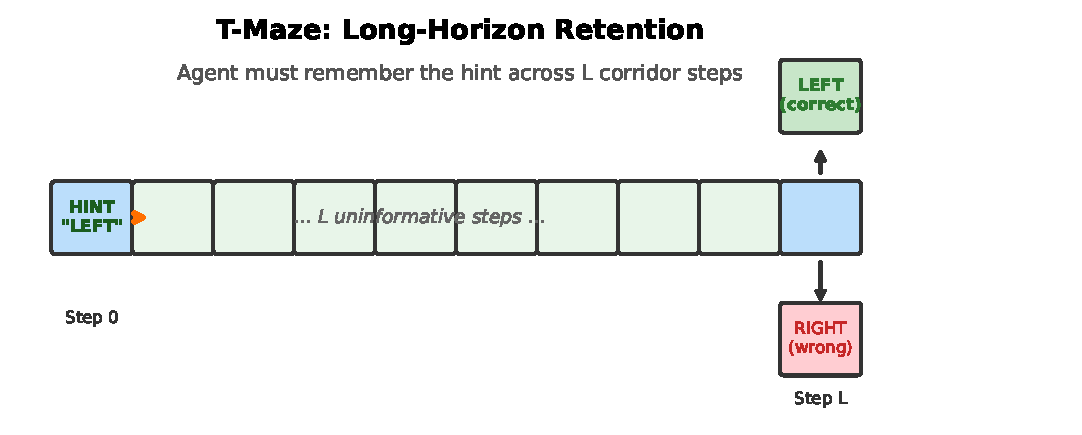
\includegraphics[width=0.85\textwidth]{diagram_tmaze.pdf}\\[2pt]
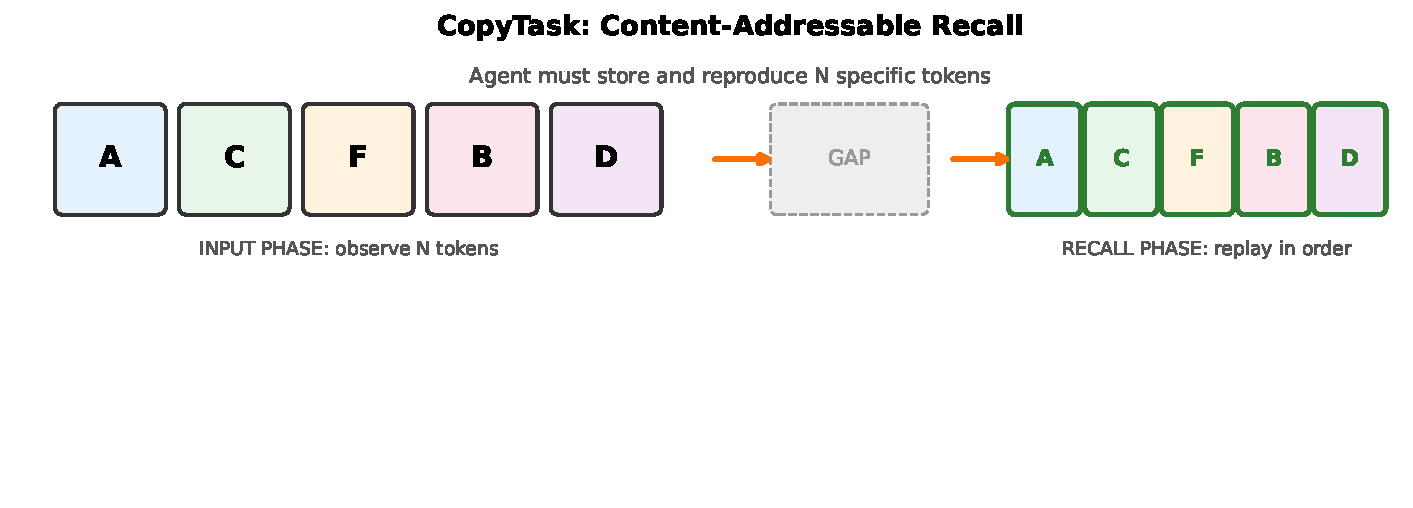
\includegraphics[width=0.85\textwidth]{diagram_copytask.pdf}
\caption{Synthetic benchmark tasks. \textbf{Top:} T-Maze --- the agent receives a hint at step~0, traverses $L$ uninformative steps, and must choose the matching direction. Tests long-horizon retention. \textbf{Bottom:} CopyTask --- the agent observes $N$ tokens, waits, then replays them in order. Tests content-addressable recall.}
\label{fig:task-diagrams}
\end{figure}

\subsection{MuJoCo POMDPs (Imperfect Teachers)}
\label{sec:mujoco-setup}

We create POMDPs from standard MuJoCo locomotion environments by removing velocity observations.
The agent observes only joint positions and must infer velocities from position history.

\paragraph{HalfCheetah-POMDP.} 8-dim positions (from 17-dim full obs), 6-dim actions.
\paragraph{Ant-POMDP.} 13-dim positions (from 27-dim), 8-dim actions.

\paragraph{MetaDrive.}
MetaDrive is an autonomous driving simulator with lidar-based observations (91-dim: 19 state dimensions + 72 lidar lasers at 50m range) and 2-dim continuous actions (steering, acceleration).
Unlike the MuJoCo POMDPs, MetaDrive is \emph{inherently} partially observable---no observation masking is needed.

The teacher for MuJoCo environments is trained on the \emph{full-observation} environment (with velocities) using RecurrentPPO~\citep{schulman2017ppo} with an LSTM backbone (\cref{fig:pipeline}).
During demonstration collection, the teacher acts using full observations, but we record only the position-masked observations that the student will see.

\begin{figure}[ht]
\centering
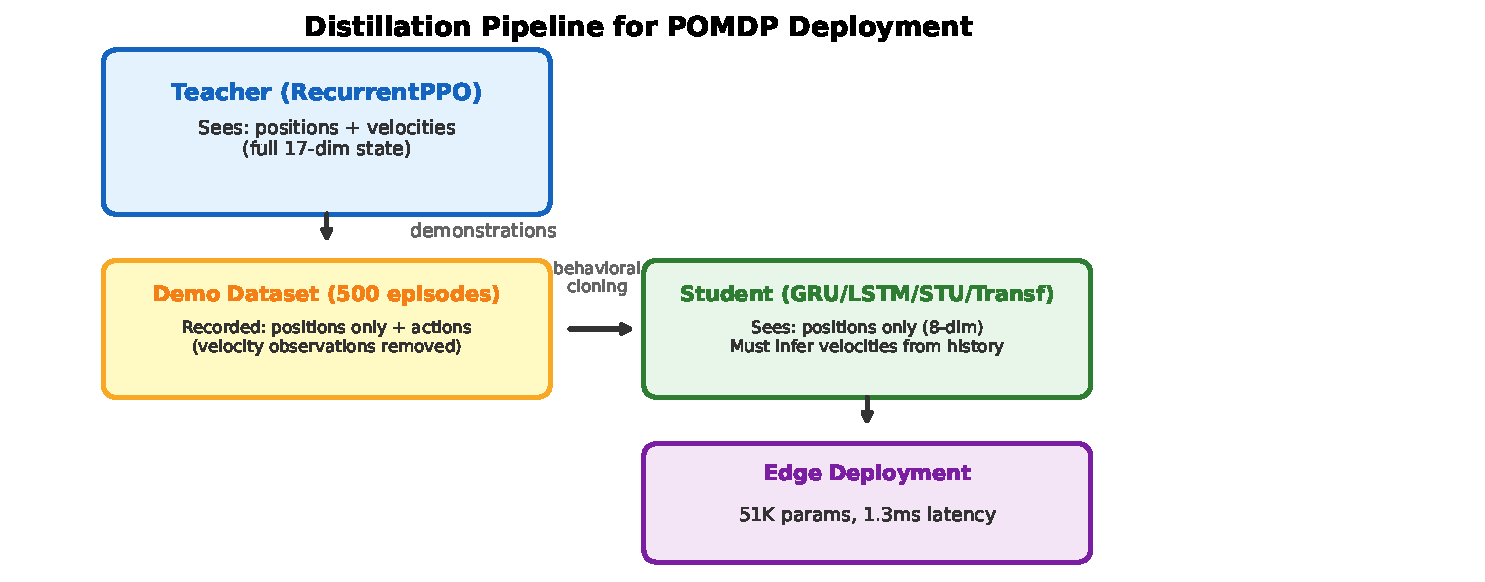
\includegraphics[width=0.8\textwidth]{diagram_pipeline.pdf}
\caption{Distillation pipeline. The teacher trains on full observations (positions + velocities), but demonstrations are recorded with only position observations. The student learns to map position histories to actions via behavioral cloning, then deploys on edge hardware.}
\label{fig:pipeline}
\end{figure}

Random baselines: HalfCheetah-POMDP $= -275 \pm 72$; Ant-POMDP $= -69 \pm 109$.

\section{Teacher Quality Manipulation}
\label{sec:teacher-quality}

We vary teacher quality along two axes:

\paragraph{Training progress.} Checkpoints at 200K, 500K, 1M, and 2M training timesteps.
\paragraph{Action noise.} Gaussian noise $\sigma \in \{0.0, 0.3\}$ added to actions during demonstration collection.

Together, these produce 8 teacher quality levels per environment, spanning returns from 210 to 1{,}424 (Ant) and 464 to 1{,}385 (HalfCheetah).

\begin{table}[ht]
\centering
\caption{Teacher return at each quality level (seed 42).}
\label{tab:teacher-quality}
\begin{tabular}{lcc}
\toprule
Teacher Configuration & HalfCheetah & Ant \\
\midrule
200K steps            & 534 & 647 \\
500K steps            & 1{,}013 & 963 \\
1M steps              & 1{,}385 & 1{,}424 \\
2M steps              & 1{,}378 & $439^*$ \\
\midrule
200K + noise $\sigma{=}0.3$ & 464 & 216 \\
500K + noise $\sigma{=}0.3$ & 592 & 251 \\
1M + noise $\sigma{=}0.3$   & 738 & 317 \\
2M + noise $\sigma{=}0.3$   & 811 & 210 \\
\bottomrule
\end{tabular}
\\[4pt]
{\small $^*$Ant teacher at 2M steps exhibits training instability.}
\end{table}

\section{Distillation Protocol}
\label{sec:distill-protocol}

For each (environment, teacher quality, student architecture, seed):
(1) collect 500 teacher episodes;
(2) split 80/20 train/val;
(3) train with MSE action loss (\cref{eq:bc}), AdamW lr${=}3{\times}10^{-4}$, cosine schedule, 100 epochs with early stopping (patience 10), gradient clipping at 1.0;
(4) evaluate: 20 rollouts in the POMDP.
We use 3 seeds (42, 123, 456) per condition; on four key conditions per environment, we run 2 additional seeds (789, 1337) for 5-seed estimates.

\section{JEPA Auxiliary Loss}
\label{sec:jepa-setup}

In addition to the action loss, we test a JEPA-style predictive latent auxiliary objective inspired by I-JEPA~\citep{assran2023ijepa} and V-JEPA~\citep{bardes2024vjepa}.
A predictor MLP takes the student's current hidden state $h_t$ and the next $k$ actions, and predicts the teacher's hidden state $k$ steps in the future:
\begin{equation}
  \loss_\text{JEPA} = \frac{1}{T-k} \sum_{t=1}^{T-k} \| f_\text{pred}(h_t, a_{t:t+k-1}) - \text{sg}(z_{t+k}^\text{teacher}) \|_2^2
\end{equation}
where $\text{sg}(\cdot)$ denotes stop-gradient and $k=5$.
The total objective is $\loss_\text{total} = \alpha \cdot \loss_\text{action} + \beta \cdot \loss_\text{hidden} + \delta \cdot \loss_\text{JEPA}$ with $\alpha=1.0$, $\beta=0.5$, $\delta \in \{0.0, 0.5\}$.


\chapter{Results}
\label{ch:results}
\section{Synthetic Benchmarks with Optimal Teachers}
\label{sec:synthetic}

We begin with controlled synthetic tasks where teacher quality is not a variable---the teacher is always optimal.
This isolates how different memory mechanisms interact with distillation.

\paragraph{T-Maze (retention).}

\begin{table}[ht]
\centering
\caption{T-Maze accuracy ($\uparrow$, max${=}1.0$) across corridor lengths. Optimal teacher, 1000 demos, 3 seeds.}
\label{tab:tmaze}
\begin{tabular}{lcccc}
\toprule
Architecture & $L=10$ & $L=50$ & $L=100$ & $L=200$ \\
\midrule
GRU            & $1.00 \pm .00$ & $1.00 \pm .00$ & $1.00 \pm .00$ & $\mathbf{1.00 \pm .00}$ \\
LSTM           & $1.00 \pm .00$ & $1.00 \pm .00$ & $1.00 \pm .00$ & $\mathbf{1.00 \pm .00}$ \\
Transformer    & $1.00 \pm .00$ & $1.00 \pm .00$ & $1.00 \pm .00$ & $0.05 \pm .02$ \\
STU-T          & $0.05 \pm .02$ & $0.05 \pm .02$ & $0.05 \pm .02$ & $0.05 \pm .02$ \\
\bottomrule
\end{tabular}
\end{table}

GRU and LSTM achieve perfect accuracy on corridors up to 200 steps---0 failures across 3 seeds each (\cref{tab:tmaze}).
Transformer succeeds up to $L{=}100$ but fails at $L{=}200$: its 64-step sliding window cannot reach the hint at step~0, a structural limitation that no amount of training data can fix.
STU-T (the tensordot approximation) fails at every corridor length, a catastrophic failure we analyze below.
With an optimal teacher and sufficient demonstrations, retention is trivially solved by any recurrent architecture---the gating mechanisms configure to preserve the hint signal without difficulty.

\paragraph{CopyTask (recall).}

\begin{table}[ht]
\centering
\caption{CopyTask: mean return ($\uparrow$, max${=}N$). 1000 demos, 3 seeds.}
\label{tab:copy-standard}
\begin{tabular}{lccc}
\toprule
Architecture & $N=5$ & $N=10$ & $N=20$ \\
\midrule
Transformer    & $3.87 \pm 0.09$ & $\mathbf{8.98 \pm 0.01}$ & $\mathbf{18.84 \pm 0.04}$ \\
GRU            & $\mathbf{4.00 \pm 0.00}$ & $\mathbf{9.00 \pm 0.00}$ & $13.60 \pm 0.57$ \\
LSTM           & $\mathbf{4.00 \pm 0.00}$ & $8.33 \pm 0.48$ & $9.78 \pm 0.38$ \\
STU-T          & $\mathbf{4.00 \pm 0.00}$ & $1.09 \pm 0.03$ & $2.31 \pm 0.07$ \\
\bottomrule
\end{tabular}
\end{table}

CopyTask reveals where architecture \emph{does} matter.
At $N{=}20$, Transformer achieves $18.84/20$ (94\%) while GRU reaches only $13.60$ (68\%) and LSTM $9.78$ (49\%).
The mechanism is structural: during recall, the Transformer directly attends to stored tokens via content-addressable lookup, bypassing the information bottleneck of a fixed-size hidden state~\citep{chen2021decision}.
This refines the picture: architecture-independence holds for \emph{retention} but not for \emph{recall}.
The relevant axis is memory mechanism, not inductive bias.

\paragraph{Data efficiency.}
On CopyTask ($N{=}10$), no architecture (excluding STU-T) shows a consistent data efficiency advantage across demonstration budgets from 5 to 1{,}000 (\cref{fig:synthetic-summary}c).
All follow similar trajectories, with Transformer pulling ahead only above 250 demonstrations due to its recall advantage.
On T-Maze ($L{=}100$), GRU achieves perfect accuracy from just 5 demonstrations, while LSTM requires 10---the only condition where architecture matters with an optimal teacher.
Adding a JEPA auxiliary loss~\citep{assran2023ijepa, lecun2022path} recovers LSTM to $1.00$ at budget${=}5$, but this is the only condition where JEPA provides a measurable benefit; across all other architectures, budgets, and tasks, JEPA shows no consistent effect (\cref{fig:jepa-null}; we note that the self-supervised JEPA sweep was conducted on STU-T, which fails independently; the teacher-supervised null on GRU, LSTM, and Transformer is the more informative result).

\begin{figure}[ht]
\centering
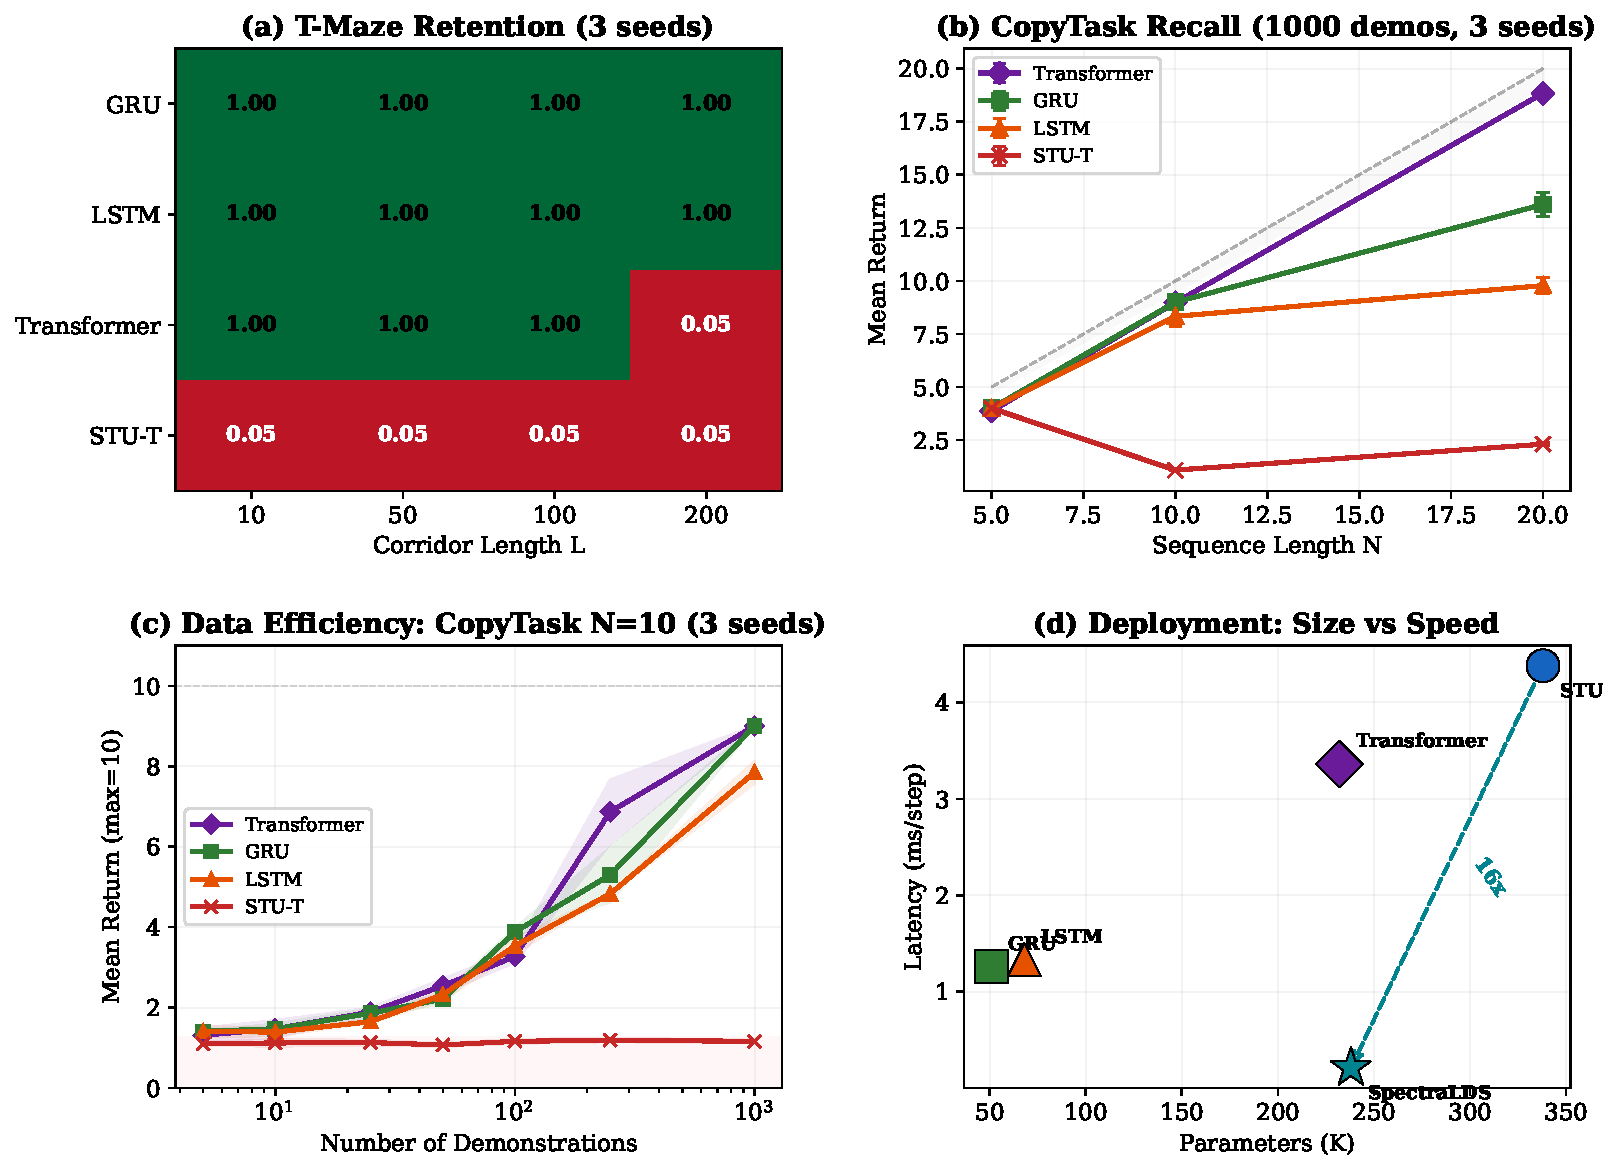
\includegraphics[width=\textwidth]{FIGURE_1_main_4panel.pdf}
\caption{\textbf{Synthetic benchmark summary.} (a)~T-Maze retention: GRU and LSTM hold the hint perfectly; Transformer fails at $L{=}200$ (window exceeded); STU-T fails everywhere. (b)~CopyTask recall: Transformer pulls away at $N{=}20$ via content-addressable lookup. (c)~Data efficiency on CopyTask $N{=}10$: all viable architectures follow similar trajectories; Transformer separates above 250 demos. (d)~Deployment trade-off: GRU and LSTM are Pareto-optimal for latency; SpectraLDS conversion yields $16\times$ speedup over full STU.}
\label{fig:synthetic-summary}
\end{figure}

\begin{figure}[ht]
\centering
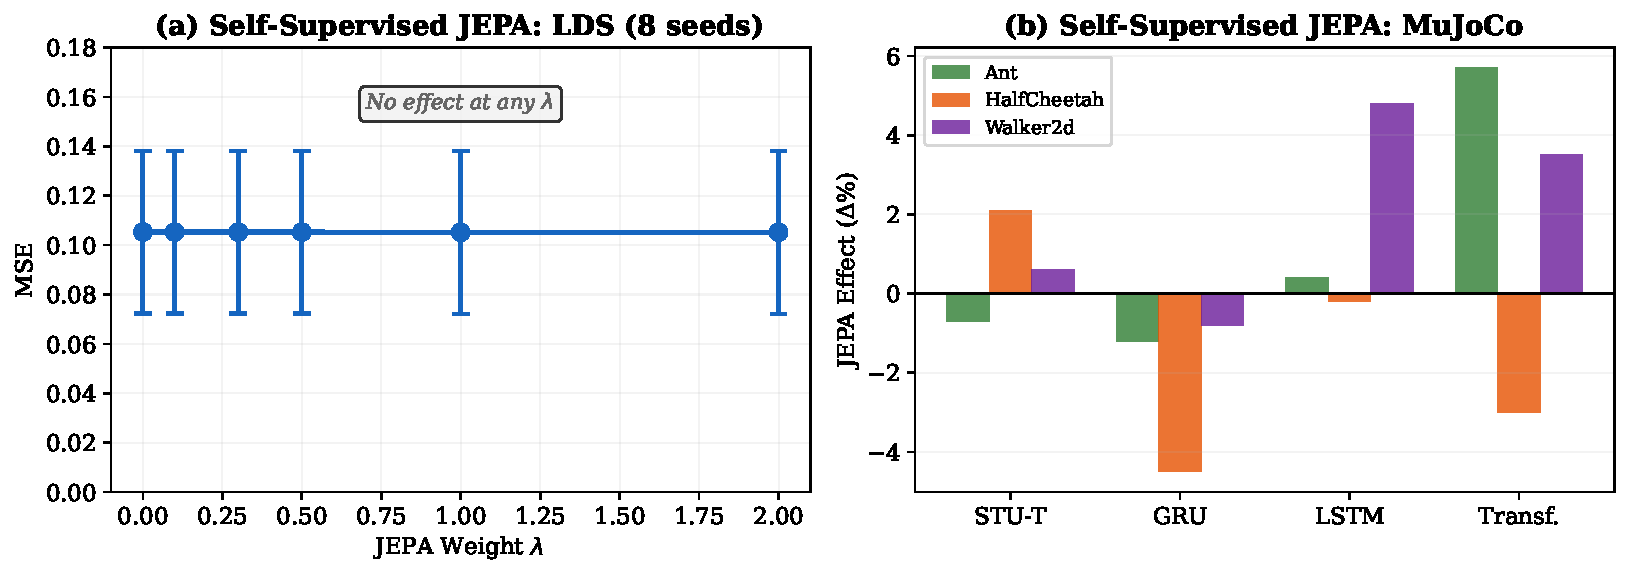
\includegraphics[width=\textwidth]{FIGURE_2_jepa_null_2panel.pdf}
\caption{\textbf{JEPA auxiliary loss produces no consistent benefit.} (a)~Self-supervised JEPA on LDS: MSE is flat at $0.105$ across all $\lambda$ values (8 seeds). (b)~Self-supervised JEPA on MuJoCo: per-architecture effect ranges from $-4.5\%$ to $+5.7\%$ with no consistent direction.}
\label{fig:jepa-null}
\end{figure}

\paragraph{STU-T tensordot failure.}
\label{sec:stu-t-failure}

\begin{table}[ht]
\centering
\caption{Flash STU LDS replication: MSE ($\downarrow$). 16 seeds. Full STU achieves substantially lower MSE (up to $40\times$ vs LSTM) than all other architectures. STU-T tensordot is worst despite using identical spectral filters.}
\label{tab:lds-replication}
\begin{tabular}{lcccc}
\toprule
Model & $\rho=0.9$ & $\rho=0.95$ & $\rho=0.99$ & $\rho=0.999$ \\
\midrule
STU (full)  & $\mathbf{.0003}$ & $\mathbf{.0004}$ & $\mathbf{.0004}$ & $\mathbf{.0003}$ \\
GRU         & $.002$ & $.002$ & $.005$ & $.008$ \\
LSTM        & $.002$ & $.002$ & $.007$ & $.012$ \\
Transformer & $.014$ & $.023$ & $.046$ & $.062$ \\
STU-T       & $.054$ & $.072$ & $.104$ & $.121$ \\
\bottomrule
\end{tabular}
\end{table}

Our STU and STU-T implementations follow the architecture described in~\citet{agarwal2024spectral} and~\citet{liu2025flashstu}, using their published hyperparameters ($K{=}16$ filters, same learning rate and optimizer) without additional tuning at our compact scale; we verified our full STU reproduces their published LDS results at $d_\text{model}{=}64$ (\cref{tab:lds-replication}).
The Flash STU tensordot approximation factorizes each filter's projection matrix $M_k \approx M^{(1)} \otimes M^{(2)}$, reducing parameters from $2K \cdot d^2$ to $2K \cdot d + d^2$.
At the Flash STU paper's scale ($d_\text{model} \geq 128$, 4+ layers), this is tight.
At our compact student scale ($d_\text{model}=64$, 2 layers), the rank-1 Kronecker constraint is catastrophic: STU-T achieves $0.104$ MSE on LDS at $\rho{=}0.99$, compared to $0.002$ published by~\citet{liu2025flashstu} at $d_\text{model}{=}128$---a $52\times$ gap, though we note the comparison is across different model scales.
Against our own full STU at the \emph{same} $d_\text{model}{=}64$, STU-T is $260\times$ worse ($0.104$ vs $0.0004$), isolating the tensordot factorization as the cause.
On all distillation tasks beyond the easiest condition (CopyTask $N{=}5$, where every architecture achieves perfect scores), STU-T scores at chance level.
Meanwhile, full STU achieves the best sequence prediction of any architecture ($5$--$27\times$ lower MSE than GRU on LDS, depending on spectral radius), confirming the spectral prior is powerful---the tensordot approximation destroys it at compact scale.
This finding is unreported in prior work~\citep{liu2025flashstu, agarwal2024spectral} and directly relevant to practitioners building compact spectral models.

\begin{figure}[ht]
\centering
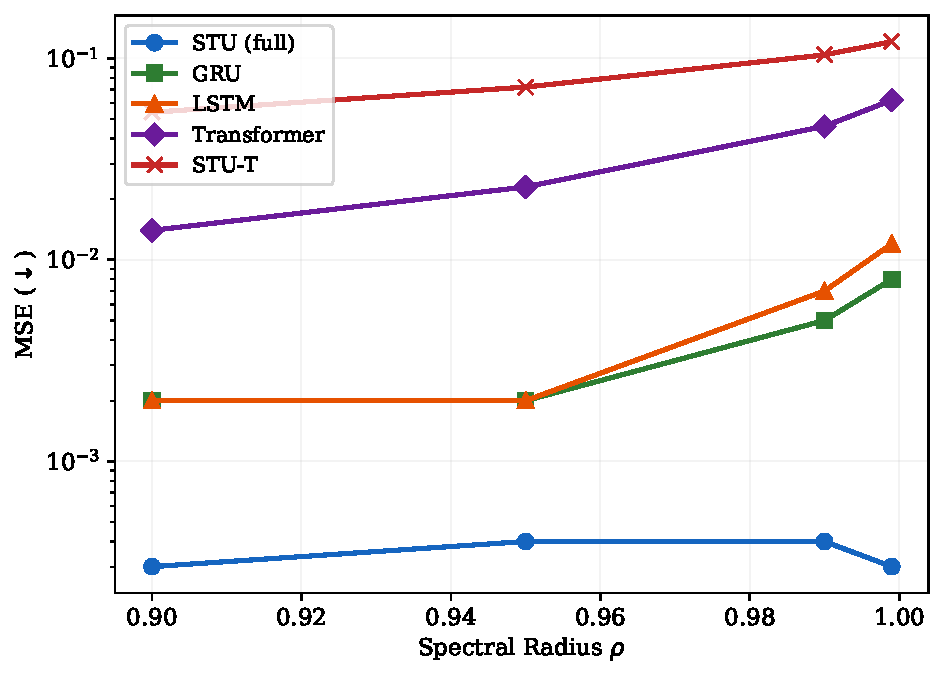
\includegraphics[width=0.5\textwidth]{FIGURE_3_lds_replication.pdf}
\caption{LDS replication (16 seeds, log scale). Full STU achieves $0.0003$ MSE. STU-T is worst at every spectral radius despite using the same spectral filters.}
\label{fig:lds-replication}
\end{figure}
\vspace{-6pt}

With optimal teachers, the synthetic benchmarks establish three points: (1) retention is trivially solved by recurrent models, (2) recall requires attention, and (3) the STU-T tensordot approximation fails catastrophically at compact scale.
The critical question is whether these patterns hold when teachers are imperfect.

\section{Continuous-Control POMDPs with Imperfect Teachers}
\label{sec:mujoco}

The synthetic results show that architecture choice is largely irrelevant when teachers are optimal.
But real-world deployment rarely involves perfect teachers.
Sim-to-real transfer introduces systematic distributional shift.
Human demonstrations are noisy and inconsistent.
Foundation model distillation involves teachers with their own errors and biases.
This chapter tests whether the architecture-independence finding survives the realistic regime of imperfect teachers.

\paragraph{Teacher quality dominates architecture choice.}


\begin{figure}[t]
\centering
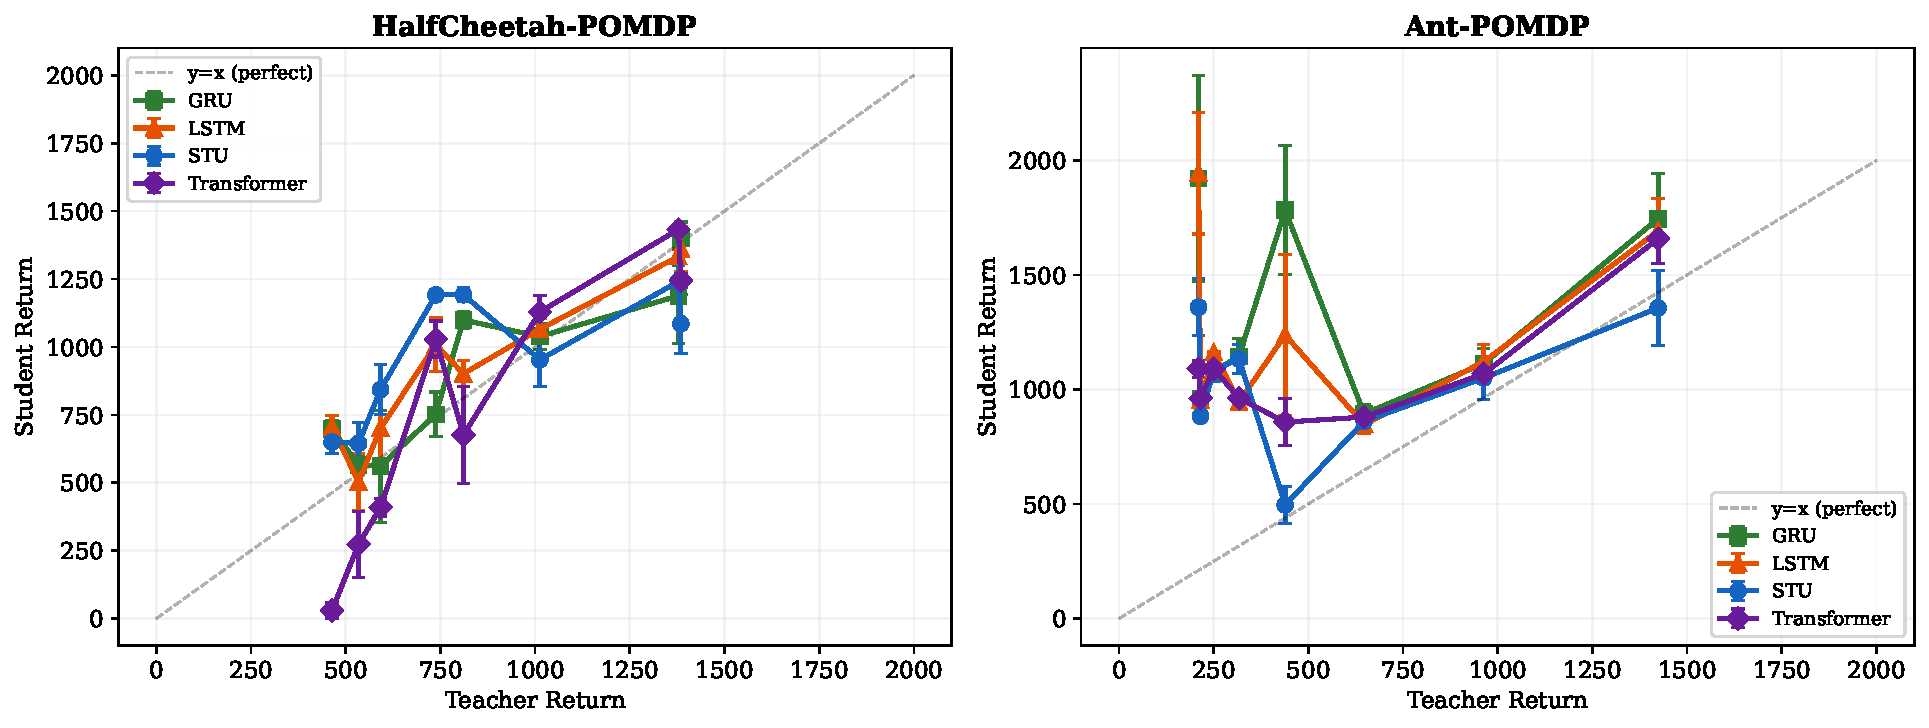
\includegraphics[width=0.9\textwidth]{FIGURE_4_mujoco_distill_efficiency.pdf}
\caption{\textbf{The key result: student return vs.\ teacher return on MuJoCo POMDPs.} Each point represents one (architecture, teacher quality) condition averaged over 3 seeds; error bars show $\pm 1$ std. Points above the dashed $y{=}x$ line indicate students that \emph{surpass} their teacher (\cref{sec:surpass}). The spread due to teacher quality (horizontal extent of each curve) far exceeds the spread due to architecture (vertical gap between curves at fixed teacher quality).}
\label{fig:distill-efficiency}
\end{figure}
\vspace{-6pt}

\Cref{fig:distill-efficiency} presents our central finding.
On both HalfCheetah and Ant POMDPs, student return is primarily determined by teacher quality, with architecture providing second-order variation.

To quantify this, we perform a two-way ANOVA decomposing student return variance into teacher quality and architecture main effects:
\begin{equation}
  R_{a,q,s} = \mu + \alpha_a + \beta_q + (\alpha\beta)_{a,q} + \epsilon_{a,q,s}
  \label{eq:anova}
\end{equation}
where $R_{a,q,s}$ is the return for architecture $a$, teacher quality $q$, and seed $s$; $\alpha_a$ is the architecture main effect; $\beta_q$ is the teacher quality main effect; $(\alpha\beta)_{a,q}$ is the interaction; and $\epsilon$ is residual.
We report $\eta^2$ (the fraction of total sum of squares explained by each factor):

\begin{table}[ht]
\centering
\caption{Two-way ANOVA: fraction of student return variance ($\eta^2$) explained by each factor. The interaction term captures how architecture effects vary with teacher quality. Error captures unexplained variance (seed-to-seed noise and unmodeled interactions).}
\label{tab:anova}
\begin{tabular}{lcccc}
\toprule
Environment & Teacher $\eta^2$ & Architecture $\eta^2$ & Interaction $\eta^2$ & Error \\
\midrule
HalfCheetah & $71.9\%$ & $4.6\%$ & $17.3\%$ & $6.1\%$ \\
Ant         & $49.1\%$ & $11.0\%$ & $25.2\%$ & $14.8\%$ \\
Ant (excl.\ 2M$^*$) & $65.8\%$ & $4.9\%$ & $16.1\%$ & $13.2\%$ \\
MetaDrive   & $58.3\%$ & $14.1\%$ & $19.7\%$ & $7.9\%$ \\
\bottomrule
\end{tabular}
\\[2pt]
{\small $^*$Ant 2M teacher exhibits training instability; see \cref{tab:ant-distill}.}
\end{table}

Across the teacher-quality range we tested, teacher quality explains substantially more variance than architecture: $72\%$ vs $5\%$ on HalfCheetah, $49\%$ vs $11\%$ on Ant, and $58\%$ vs $14\%$ on MetaDrive.
The interaction term ($17$--$25\%$) is also substantial, reflecting that architecture differences are amplified under poor teacher quality---consistent with our qualitative findings in \cref{sec:arch-patterns}.
Excluding the pathological Ant 2M teacher (which is an unstable single-seed checkpoint), the teacher-quality $\eta^2$ rises to $66\%$ and the architecture $\eta^2$ drops to $5\%$.

We note that $\eta^2$ is sensitive to how widely each factor is manipulated: we varied teacher return over a ${\sim}7\times$ range (210--1{,}424) while comparing only 4 architectures at fixed $d_\text{model}$.
The absolute $\eta^2$ values should be interpreted as characterizing the relative importance of these factors \emph{across the specific experimental range we studied}, not as universal constants.

The substantial interaction term has an important practical implication: our recommendation to prioritize teacher quality applies most strongly when the practitioner \emph{can} improve the teacher.
When the teacher is fixed and imperfect---e.g., when learning from human demonstrations or a pre-trained foundation model---architecture selection becomes more consequential, and the patterns in \cref{sec:arch-patterns} become the relevant guide.

The practical implication is direct: a practitioner's compute budget has far more impact when spent training a better teacher than when spent searching for a better student architecture.





\begin{table}[ht]
\centering
\caption{HalfCheetah-POMDP: student return (mean $\pm$ std). $\dagger$ = 5 seeds; all others 3 seeds. Random baseline: $-275 \pm 72$. MLP and FrameStack (FS) are non-temporal baselines.}
\label{tab:hc-distill}
\resizebox{\textwidth}{!}{%
\begin{tabular}{lrcccccc}
\toprule
Teacher Config & Ret. & MLP & FS & GRU & LSTM & STU & Transformer \\
\midrule
200K           & 534  & $-33$ & $-16$ & $565{\pm}36$  & $503{\pm}106$ & $\mathbf{645{\pm}78}$  & $274{\pm}121$ \\
500K           & 1013 & $-78$ & $-38$ & $1039{\pm}49$ & $1065{\pm}40$ & $953{\pm}98$  & $\mathbf{1129{\pm}62}$ \\
1M$^\dagger$   & 1385 & $-68$ & $-53$ & $\mathbf{1401{\pm}59}$  & $1359{\pm}83$ & $1086{\pm}108$ & $1245{\pm}25$ \\
2M$^\dagger$   & 1378 & $-55$ & $-14$ & $1188{\pm}175$ & $1333{\pm}27$ & $1241{\pm}61$ & $\mathbf{1433{\pm}7}$ \\
\midrule
200K+n$^\dagger$ & 464  & $-18$ & $-9$ & $698{\pm}30$  & $\mathbf{703{\pm}44}$  & $650{\pm}43$  & $30{\pm}29$ \\
500K+n         & 592  & $-23$ & $-24$ & $561{\pm}206$ & $702{\pm}143$ & $\mathbf{843{\pm}91}$  & $410{\pm}32$ \\
1M+n           & 738  & $-39$ & $19$ & $752{\pm}82$  & $1008{\pm}99$ & $\mathbf{1191{\pm}11}$ & $1028{\pm}68$ \\
2M+n$^\dagger$ & 811  & $-39$ & $250$ & $1099{\pm}30$ & $901{\pm}47$  & $\mathbf{1192{\pm}27}$ & $676{\pm}178$ \\
\bottomrule
\end{tabular}
}
\end{table}

\begin{table}[ht]
\centering
\caption{Ant-POMDP: student return (mean $\pm$ std). $\dagger$ = 5 seeds; all others 3 seeds. Random baseline: $-69 \pm 109$. On Ant, MLP and FrameStack are competitive with temporal models---memory provides only modest benefit.}
\label{tab:ant-distill}
\resizebox{\textwidth}{!}{%
\begin{tabular}{lrcccccc}
\toprule
Teacher Config & Ret. & MLP & FS & GRU & LSTM & STU & Transformer \\
\midrule
200K           & 647  & $959$ & $942$ & $894{\pm}40$  & $847{\pm}38$  & $861{\pm}42$  & $\mathbf{879{\pm}18}$ \\
500K           & 963  & $1041$ & $1041$ & $1112{\pm}66$ & $\mathbf{1121{\pm}73}$ & $1050{\pm}92$ & $1068{\pm}35$ \\
1M$^\dagger$   & 1424 & $1129$ & $1042$ & $\mathbf{1745{\pm}195}$ & $1692{\pm}141$ & $1356{\pm}165$ & $1657{\pm}108$ \\
2M$^{*,\dagger}$ & 439  & $1408$ & $1307$ & $\mathbf{1783{\pm}283}$ & $1238{\pm}351$ & $496{\pm}81$   & $858{\pm}103$ \\
\midrule
200K+n$^\dagger$ & 216  & $963$ & $954$ & $961{\pm}13$  & $952{\pm}5$   & $883{\pm}17$  & $\mathbf{961{\pm}7}$ \\
500K+n         & 251  & $1012$ & $967$ & $1079{\pm}45$ & $\mathbf{1161{\pm}3}$  & $1083{\pm}48$ & $1090{\pm}37$ \\
1M+n           & 317  & $980$ & $956$ & $\mathbf{1145{\pm}76}$  & $945{\pm}18$  & $1134{\pm}63$ & $962{\pm}23$ \\
2M+n$^\dagger$ & 210  & $836$ & $924$ & $1921{\pm}450$ & $\mathbf{1944{\pm}265}$ & $1359{\pm}125$ & $1091{\pm}37$ \\
\bottomrule
\end{tabular}
}
\\[4pt]
{\small $^*$Ant 2M teacher exhibits training instability: this checkpoint is worse than 1M.}
\end{table}


\paragraph{Architecture patterns under imperfect teachers.}
\label{sec:arch-patterns}

While teacher quality dominates the overall variance, architecture does matter---and the pattern of differentiation is consistent and interpretable.
Three findings emerge from the full results (\cref{tab:hc-distill,tab:ant-distill}):

\paragraph{GRU is the most robust student.}
GRU achieves the highest return in 5 of 16 conditions and is within one standard deviation of the best in 10 of 16---the most consistent of any architecture (LSTM and STU tie at 8/16 near-highest, Transformer at 6/16). GRU's clearest advantages emerge under noisy or unstable teachers; on clean, moderate-quality teachers, most architectures perform comparably. GRU is also the smallest (51K params) and fastest (1.26\,ms/step, sufficient for 800\,Hz control loops) temporal architecture.
On Ant, GRU dominates: 1{,}745 at 1M (highest), 1{,}783 at 2M (highest), 1{,}145 at 1M+noise (highest).
The parameter-matched comparison (\cref{sec:param-matched}) confirms this is a genuine architectural advantage, not a capacity artifact: GRU$_{160}$ at 312K params outperforms STU at 338K params (overall mean $1{,}222$ vs $1{,}001$), and additional capacity actually \emph{improves} GRU performance (GRU$_{160}$ overall $1{,}222$ vs GRU$_{64}$ overall $1{,}122$).

\paragraph{Transformer is the most volatile.}
With high-quality teachers, Transformer performs well: $1{,}433$ on HalfCheetah 2M (the best), $1{,}657$ on Ant 1M.
With low-quality noisy teachers, it collapses: \textbf{30} on HalfCheetah 200K+noise---barely above random ($-275$).
Parameter count alone does not explain this: GRU$_{160}$ (312K params) shows no similar collapse, suggesting that attention's lack of a temporal bottleneck makes it more susceptible to fitting spurious correlations in noisy demonstrations.

\paragraph{STU shows environment-specific noise robustness.}
On HalfCheetah, STU excels with noisy teachers: $1{,}191$ and $1{,}192$ at 1M/2M+noise (both highest).
On Ant, STU struggles with the unstable 2M teacher ($496$, near the teacher's $439$).
The spectral filters may provide temporal smoothing that helps on simpler dynamics (HalfCheetah, planar, 6 actions) but not on more complex ones (Ant, 3D, 8 actions).
Alternatively, STU's larger parameter count (338K) may interact differently with the two environments' observation dimensions (8 vs.\ 13).

\begin{figure}[ht]
\centering
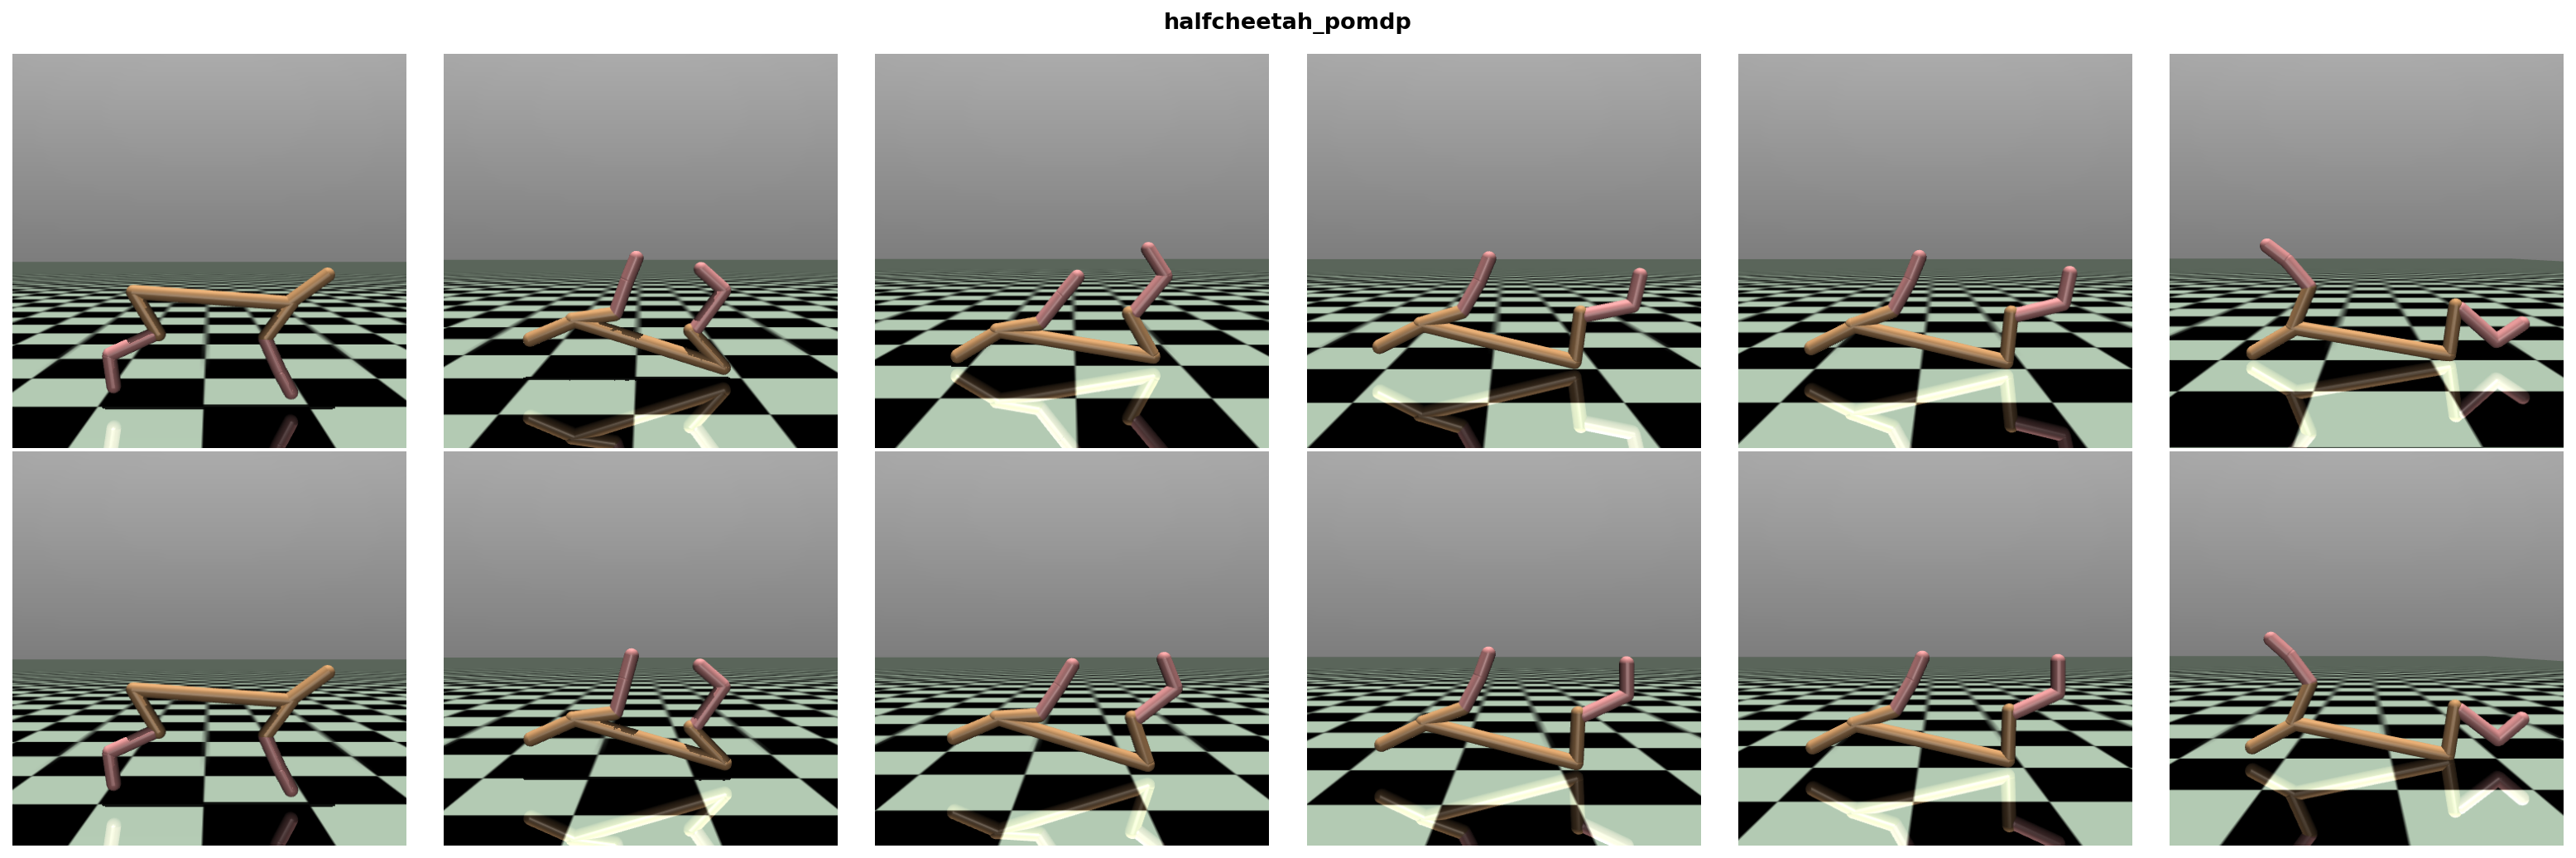
\includegraphics[width=0.6\textwidth]{RENDER_halfcheetah_best_vs_worst.png}
\vspace{-6pt}
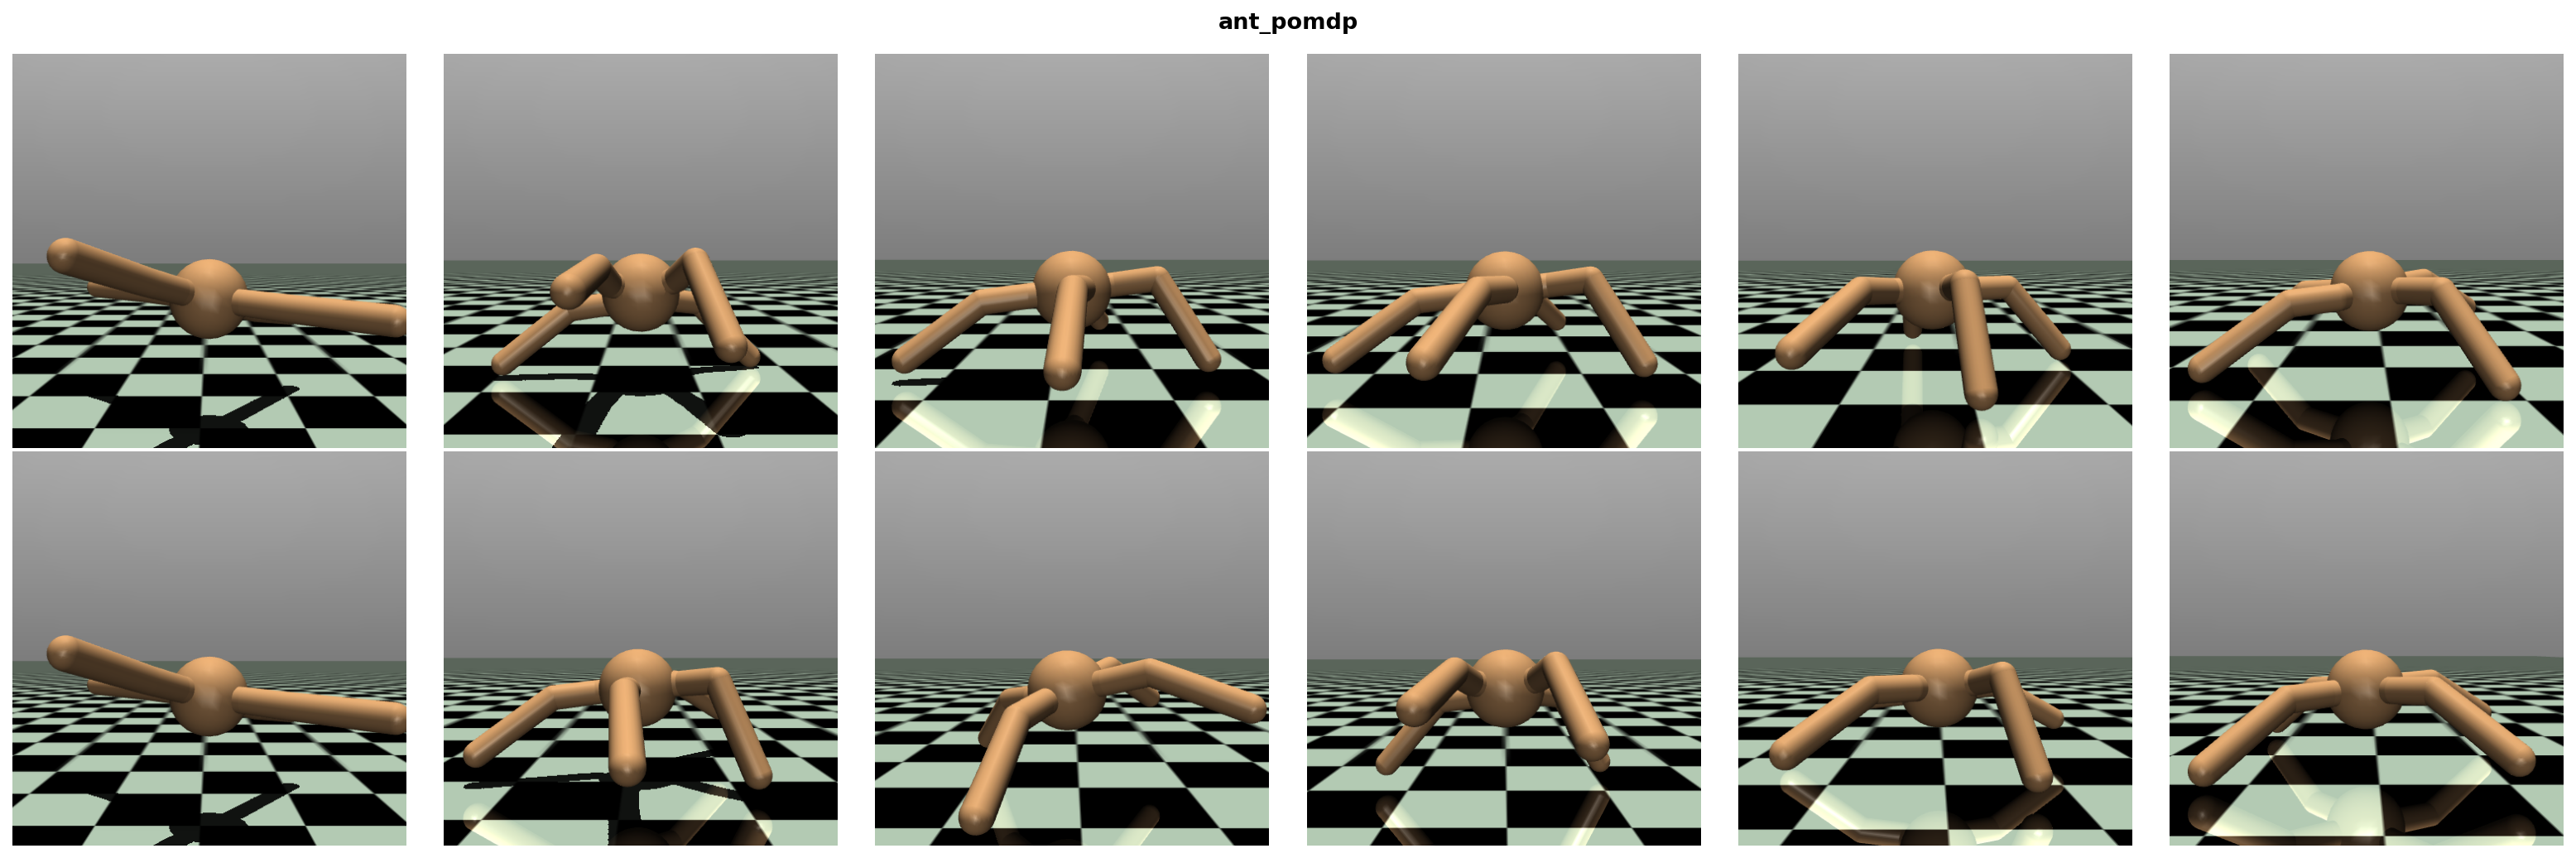
\includegraphics[width=0.6\textwidth]{RENDER_ant_best_vs_worst.png}
\caption{\textbf{Architecture differentiation under poor teachers.} Top: HalfCheetah with 200K+noise teacher---GRU (return 698) runs with a natural gait while Transformer (return 30) barely moves, consistent with Transformer's volatility under noisy demonstrations. Bottom: Ant with the unstable 2M teacher---GRU (return 1,783) walks forward while STU (return 496) collapses. }
\label{fig:mujoco-renders}
\end{figure}

\paragraph{Students frequently exceed imperfect teachers.}
\label{sec:surpass}

A striking pattern in \cref{fig:distill-efficiency}: students frequently exceed their imperfect teachers in absolute return---a phenomenon also observed in imitation learning from mixed-quality demonstrations~\citep{beliaev2022ileed}.
With the well-trained 1M teacher on Ant (return 1{,}424), GRU achieves 1{,}745---a $1.23\times$ improvement.
Ratios are larger with degraded teachers, but this primarily reflects low baselines rather than exceptional student performance.

We attribute this to two factors, neither causally tested.
First, \emph{variance averaging}: the Ant 2M teacher has high episode variance (returns 17--1{,}928, mean 439, std 368), and BC's MSE loss fits the central tendency of this distribution, producing a smoother policy that avoids the teacher's worst failure modes.
Second, \emph{implicit timestep weighting}: since BC sums loss over timesteps, longer (more successful) episodes contribute proportionally more gradient signal.
In the Ant 2M dataset, the top 15\% of episodes (return ${>}800$) contribute ${\sim}30\%$ of total timesteps, so the student disproportionately learns from the teacher's best behavior.
An episode-length-normalized BC ablation would be needed to establish causality.
The practical implication: teacher quality determines the \emph{floor}, not the ceiling, of student performance.


\paragraph{Do these tasks require memory?}
\label{sec:baselines}

To test whether our POMDP tasks genuinely require temporal reasoning, we evaluate two non-temporal baselines: an MLP that processes each observation independently, and a FrameStack model that concatenates the 8 most recent frames.

\begin{table}[ht]
\centering
\caption{Baseline comparison: mean student return across all teacher quality levels (3 seeds). Random baselines: HalfCheetah $= -275$, Ant $= -69$.}
\label{tab:baselines}
\begin{tabular}{lcc}
\toprule
Architecture & HalfCheetah-POMDP & Ant-POMDP \\
\midrule
MLP (5K)         & $-44 \pm 22$    & $1{,}041 \pm 191$ \\
FrameStack (9K)  & $15 \pm 120$    & $1{,}017 \pm 185$ \\
\midrule
GRU (51K)        & $913 \pm 317$   & $1{,}330 \pm 447$ \\
LSTM (68K)       & $947 \pm 308$   & $1{,}238 \pm 388$ \\
STU (338K)       & $975 \pm 223$   & $1{,}028 \pm 310$ \\
Transformer (232K) & $778 \pm 502$ & $1{,}071 \pm 326$ \\
\bottomrule
\end{tabular}
\end{table}

The results reveal a striking environment-dependent pattern:

\paragraph{HalfCheetah: memory is essential.}
MLP achieves $-44$ and FrameStack achieves $15$---both barely above the random baseline of $-275$ and far below every temporal architecture ($778$--$975$).
The large gap between baselines and temporal models confirms that HalfCheetah velocity inference genuinely requires integrating position history over time.
The 8-frame window of FrameStack provides crude finite-difference velocity estimates, but these are too noisy for effective locomotion.

\paragraph{Ant: memory provides modest benefit.}
MLP achieves $1{,}041$ --- a finding that echoes \citet{emmons2022rvs}, who showed simple MLPs often match fancier architectures in offline supervised RL --- and FrameStack achieves $1{,}017$---competitive with STU ($1{,}028$) and Transformer ($1{,}071$), though below GRU ($1{,}330$) and LSTM ($1{,}238$).
Ant's 13-dimensional position observations apparently contain enough information for a reactive policy to produce reasonable locomotion without explicit velocity estimation.
This strengthens our teacher-quality-dominates finding on Ant: if even the gap between \emph{no memory} and \emph{full temporal model} is modest, then the gap \emph{between} temporal architectures is necessarily small relative to teacher quality effects.

\paragraph{Parameter-matched comparison.}
\label{sec:param-matched}

The $6.6\times$ parameter gap between GRU (51K) and STU (338K) is the largest confound in our architecture comparisons.
To disentangle architecture from capacity, we train GRU at $d_\text{model} = 160$ (312K parameters), closely matching STU's 338K.

\begin{table}[ht]
\centering
\caption{Parameter-matched comparison on selected conditions (3 seeds).}
\label{tab:param-matched}
\begin{tabular}{llccc}
\toprule
Env & Teacher & GRU$_{64}$ (51K) & GRU$_{160}$ (312K) & STU (338K) \\
\midrule
\multirow{3}{*}{HC} & 1M           & $1401 \pm 59$   & $1400 \pm 33$   & $1086 \pm 108$ \\
                    & 200K+noise   & $698 \pm 30$    & $617 \pm 8$     & $650 \pm 43$ \\
                    & 2M+noise     & $1099 \pm 30$   & $1163 \pm 15$   & $1192 \pm 27$ \\
\midrule
\multirow{3}{*}{Ant} & 1M          & $1745 \pm 195$  & $\mathbf{1981 \pm 42}$   & $1356 \pm 165$ \\
                     & 200K+noise  & $961 \pm 13$    & $907 \pm 62$    & $883 \pm 17$ \\
                     & 2M+noise    & $1921 \pm 450$  & $\mathbf{2354 \pm 80}$   & $1359 \pm 125$ \\
\midrule
\multicolumn{2}{l}{Overall mean}   & $1{,}122$ & $1{,}222$ & $1{,}001$ \\
\bottomrule
\end{tabular}
\end{table}

The results decisively resolve the capacity confound.
GRU$_{160}$ (312K params) \textbf{outperforms STU (338K params) at matched capacity}: overall mean $1{,}222$ vs $1{,}001$.
On the strongest Ant conditions, GRU$_{160}$ achieves $1{,}981$ (1M teacher) and $2{,}354$ (2M+noise)---the highest returns of any model in our entire study.

GRU$_{160}$ also matches or exceeds GRU$_{64}$ in most conditions, indicating that GRU's robustness at $d_\text{model}=64$ was \emph{not} simply overfitting resistance from low capacity---more capacity actually helps GRU.
The exception is the weakest teacher condition (200K+noise), where GRU$_{64}$ slightly outperforms GRU$_{160}$ ($698$ vs $617$ on HalfCheetah), consistent with mild overfitting when both teacher quality and demonstration count are low.

\textbf{Conclusion:} GRU's advantage over STU is genuinely architectural, not a capacity artifact.
The learned gating mechanism outperforms the fixed spectral prior for policy distillation at matched parameter budgets.

\paragraph{Demo count ablation.}
\label{sec:demo-ablation}

To test whether data efficiency patterns from CopyTask hold in continuous control, we ablate the demonstration count using the 1M teacher (no noise) on both MuJoCo environments.

\begin{table}[ht]
\centering
\caption{Demo count ablation: student return with 50, 200, and 2{,}000 demonstrations (1M teacher, no noise, 3 seeds). Compare with the default 500-demo results in \cref{tab:hc-distill,tab:ant-distill} (1M row).}
\label{tab:demo-ablation}
\begin{tabular}{llcccc}
\toprule
Env & Demos & GRU & LSTM & STU & Transformer \\
\midrule
\multirow{3}{*}{HC}
 & 50    & $112 \pm 172$  & $635 \pm 228$  & $398 \pm 319$   & $-48 \pm 18$ \\
 & 200   & $916 \pm 283$  & $920 \pm 186$  & $1164 \pm 143$  & $1228 \pm 14$ \\
 & 2{,}000 & $\mathbf{1402 \pm 38}$  & $1381 \pm 61$  & $1253 \pm 88$  & $1378 \pm 40$ \\
\midrule
\multirow{3}{*}{Ant}
 & 50    & $972 \pm 49$   & $918 \pm 10$   & $919 \pm 11$    & $1054 \pm 71$ \\
 & 200   & $990 \pm 205$  & $1003 \pm 127$ & $911 \pm 33$    & $\mathbf{1486 \pm 71}$ \\
 & 2{,}000 & $1861 \pm 116$ & $\mathbf{1882 \pm 106}$ & $1497 \pm 72$ & $1181 \pm 85$ \\
\bottomrule
\end{tabular}
\end{table}

At 50 demos on HalfCheetah, LSTM ($635$) dramatically outperforms GRU ($112$) and Transformer ($-48$).
At 2{,}000 demos, all architectures converge to $1{,}253$--$1{,}402$.
This complicates our central claim: at high demonstration counts, teacher quality dominates and architecture washes out, but at low counts ($\leq 50$), architecture matters sharply.
Practitioners with limited demonstrations should invest more effort in architecture selection.

\section{MetaDrive: Beyond Locomotion}
\label{sec:metadrive}

MetaDrive is an autonomous driving simulator with lidar observations (91-dim) and continuous steering/acceleration actions.
Unlike MuJoCo POMDPs, MetaDrive is \emph{inherently} partially observable---no observation masking is needed.
Teachers were trained via RecurrentPPO for 1M steps with checkpoints at 100K, 300K, 500K, and 1M; each checkpoint was evaluated with and without action noise ($\sigma{=}0.3$), producing 8 teacher quality levels matching the MuJoCo protocol.
Teacher returns range from $32.0 \pm 16.3$ (100K) to $101.5 \pm 42.7$ (500K, the best), with the 1M checkpoint exhibiting training instability ($75.7 \pm 40.4$)---a pattern also observed in the Ant 2M teacher.

\begin{table}[ht]
\centering
\caption{MetaDrive: student return by architecture (mean across all 8 teacher configs, 5 seeds each). 240 total experiments.}
\label{tab:metadrive}
\begin{tabular}{lrr}
\toprule
Architecture & Mean Return & $\pm$ Std \\
\midrule
STU (343K)        & $\mathbf{75.4}$ & $28.2$ \\
Transformer (237K) & $73.7$ & $20.3$ \\
LSTM (72K)        & $70.0$ & $17.9$ \\
FrameStack (51K)  & $67.7$ & $23.4$ \\
GRU (56K)         & $61.5$ & $21.6$ \\
MLP (10K)         & $16.4$ & $29.0$ \\
\bottomrule
\end{tabular}
\end{table}

MetaDrive reveals a different architecture ranking from MuJoCo: STU ($75.4$) and Transformer ($73.7$) lead, followed by LSTM ($70.0$) and GRU ($61.5$).
This reversal is consistent with MetaDrive's observation structure.
MuJoCo POMDPs require integrating a short history of low-dimensional joint positions to estimate velocities---a task well-suited to GRU's compact hidden state.
MetaDrive's 91-dimensional lidar observations encode the spatial layout of roads, vehicles, and obstacles---richer structure that the STU's spectral decomposition and the Transformer's content-addressable attention can exploit more effectively than a simple gated recurrence.
The practical implication is that the ``best'' architecture depends on the observation structure: GRU for compact position-based POMDPs, STU or Transformer when the observation space carries more spatial structure.

Critically, the teacher-quality-dominates finding still holds: teacher quality range ($61.0$) is $1.7\times$ the architecture range ($35.0$), consistent with the $1.7$--$2.2\times$ ratios on MuJoCo POMDPs.
The weakest teacher (100K, return $32$) produces students averaging $35$, while the best teachers (300K--500K+noise) produce students averaging $80$--$86$---a much larger effect than switching architectures at any fixed teacher quality level.

Also notable: MLP ($16.4$) performs substantially worse than temporal architectures ($61$--$75$) on MetaDrive, unlike Ant where MLP was competitive.
This confirms that MetaDrive's lidar-based partial observability genuinely requires temporal reasoning---the agent must track vehicle trajectories over time to make safe driving decisions.

\begin{figure}[ht]
\centering
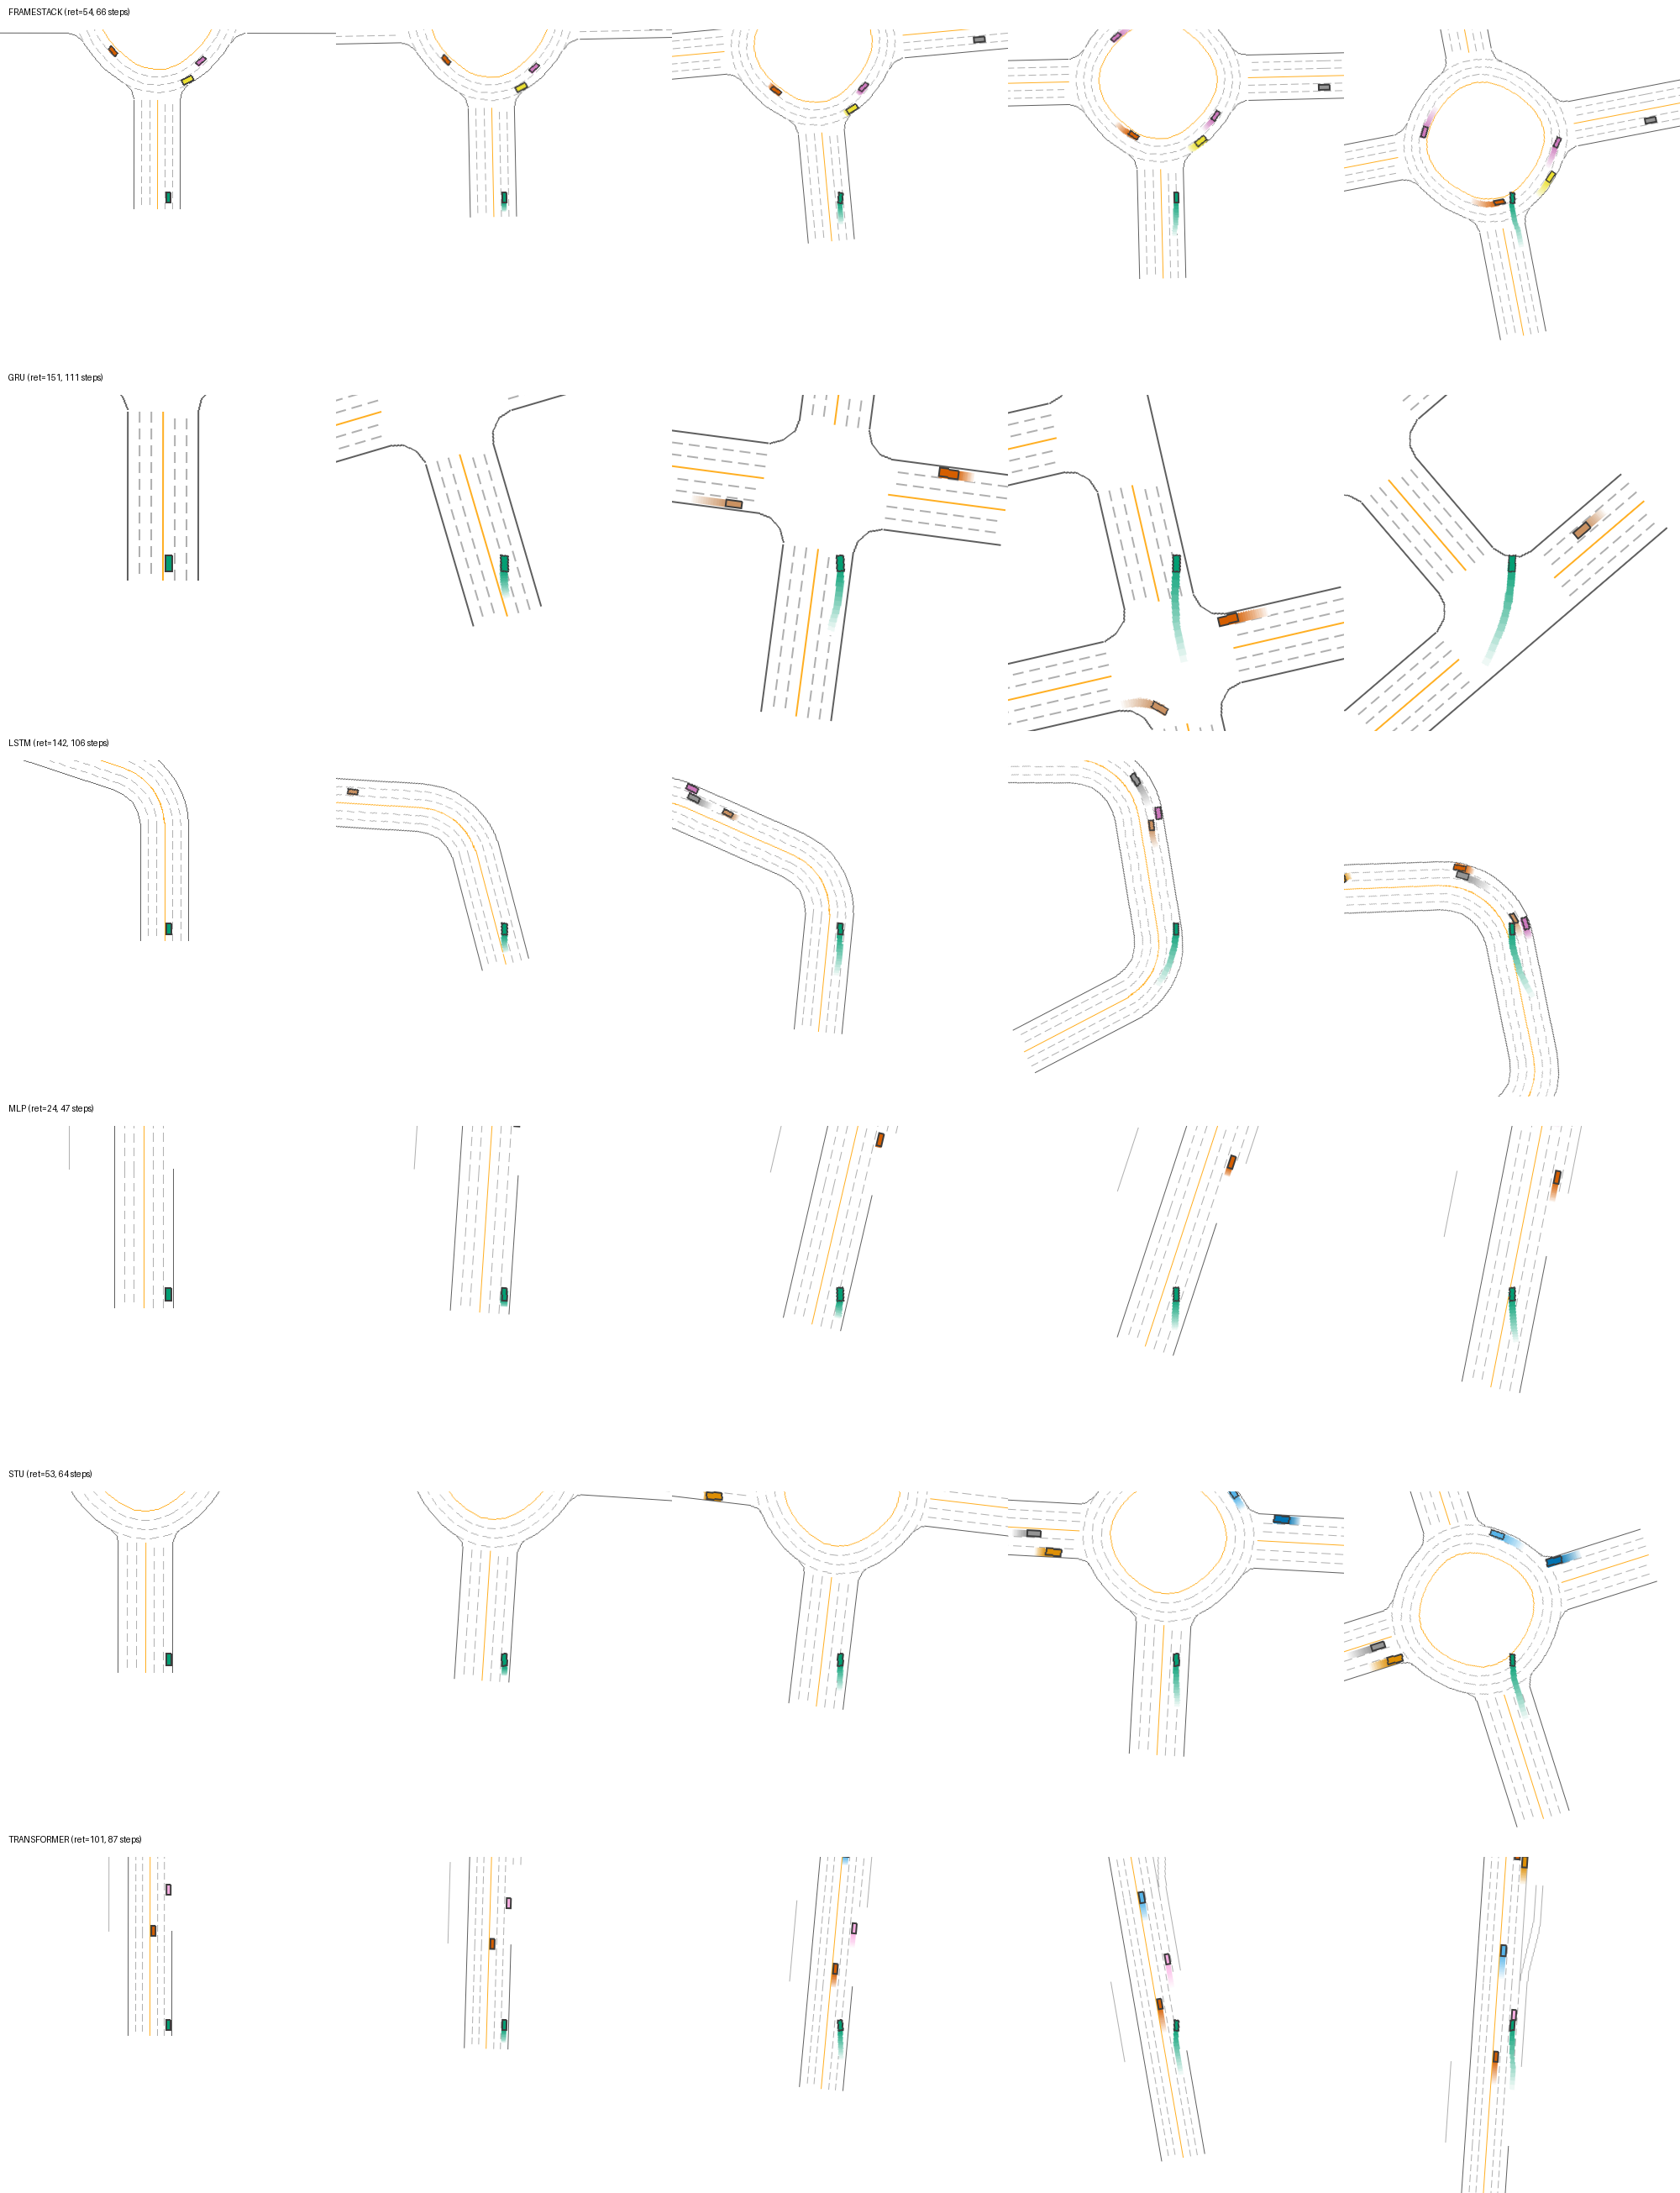
\includegraphics[width=0.7\textwidth]{comparison_metadrive_all.png}
\caption{\textbf{MetaDrive: architecture determines driving competence.} Top-down renderings of a single rollout per architecture (seed 42, 500K teacher). Each row is one architecture; columns show progression through the episode. GRU (row 2, return 151) and LSTM (row 3, return 142) navigate intersections and curves for 100+ steps. MLP (row 5, return 24) drives off-road within 47 steps, confirming that lidar-based driving requires temporal memory. STU (row 4, return 53) crashes at 64 steps despite leading in mean return across all teacher configs (\cref{tab:metadrive})---illustrating that single-rollout visualizations are anecdotal (included for visual intuition only); the table means are the authoritative comparison.}
\label{fig:metadrive-renders}
\end{figure}
\vspace{-6pt}




Video demonstrations of each architecture's locomotion and driving are available at the project repository (\url{https://github.com/wasumayan/wasumind}).


\paragraph{Deployment profiling.}
\label{sec:deployment}

Given our finding that teacher quality matters more than architecture, student selection should be driven by deployment constraints.
For locomotion tasks, GRU is the strongest deployment choice among temporal architectures: fewest parameters (51K), lowest latency (1.26\,ms/step, sufficient for 800\,Hz control loops), and the most robust distillation performance.
Full deployment profiling including latency benchmarks for all architectures is provided in \cref{app:hyperparams}.


\chapter{Discussion and Conclusion}
\label{ch:discussion}

If distillation is just supervised learning on expert demonstrations, then the student's architecture should matter less than it does in RL---and the quality of the training data (the teacher's demonstrations) should matter more.
That is exactly what we find.
Across all three environments and across the specific factor ranges we manipulated, teacher quality consistently explains more variance ($49$--$72\%$) than architecture ($5$--$14\%$).
The teacher is the signal; the architecture is the antenna.
A bad signal cannot be rescued by a fancier antenna, but a strong signal comes through on almost any receiver.

The interaction term ($17$--$25\%$) adds an important nuance: architecture matters most when teachers are worst.
When the teacher is good, any reasonable temporal architecture will learn the policy.
When the teacher is fixed and imperfect---as when learning from human demonstrations or a pre-trained foundation model---architecture selection becomes the practitioner's primary lever, and the right axis for this choice is \emph{memory mechanism}: the computational structure by which an architecture stores and retrieves temporal information.

For \textbf{retention tasks} (maintaining a signal over time), recurrent gating suffices: GRU and LSTM achieve perfect distillation from as few as 5 demonstrations.
For \textbf{recall tasks} (retrieving specific items by content), attention provides a structural advantage that no recurrent model can match.
For \textbf{temporal inference tasks} (integrating observations to estimate hidden state), the ranking is task-dependent: GRU leads on MuJoCo locomotion, but STU and Transformer lead on MetaDrive driving.
This last finding is important---it means our practical recommendations are conditional on task structure, not universal prescriptions.

\begin{figure}[ht]
\centering
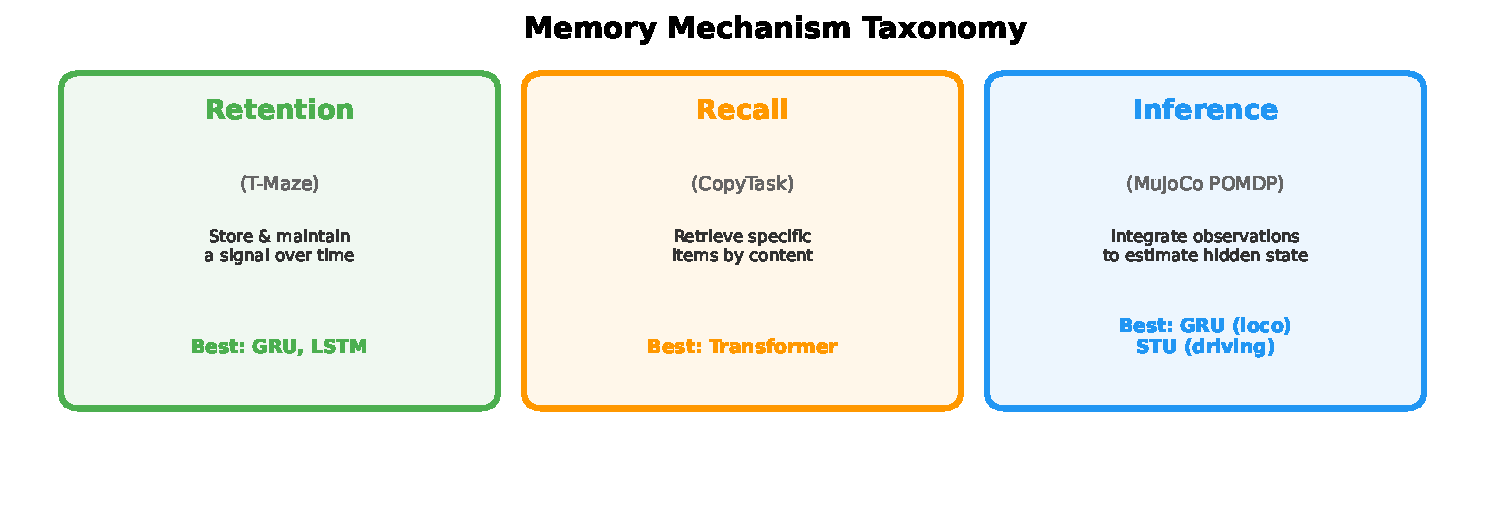
\includegraphics[width=0.85\textwidth]{diagram_taxonomy.pdf}
\caption{Memory mechanism taxonomy. The best architecture depends on the task category, but teacher quality is the dominant factor within each.}
\label{fig:taxonomy}
\end{figure}

Two additional findings deserve note.
First, full STU achieves $5$--$27\times$ lower MSE than GRU on LDS sequence prediction yet does not translate this to distillation, where GRU outperforms STU overall---better sequence prediction does not imply better policy distillation.
Relatedly, the Flash STU tensordot approximation fails catastrophically at compact scale ($d_\text{model}{=}64$), destroying the spectral prior through rank-1 Kronecker constraints.
This is unreported in prior work and directly actionable for practitioners.
Second, self-supervised JEPA provides no benefit for temporal models (likely due to unstable prediction targets), and teacher-supervised JEPA offers only marginal improvement.

\begin{figure}[ht]
\centering
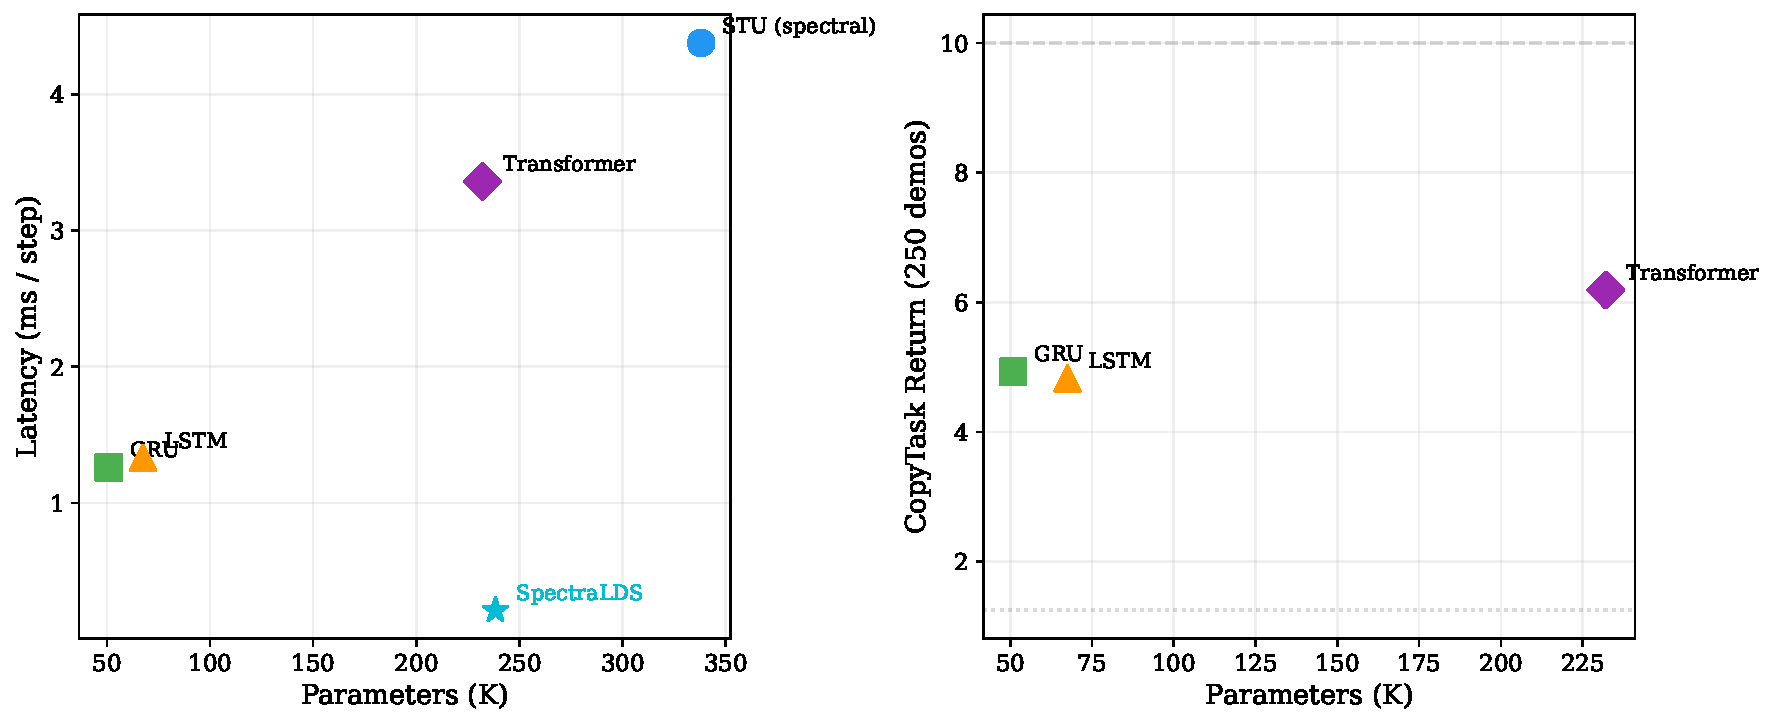
\includegraphics[width=0.65\textwidth]{FIGURE_5_deployment_scatter.pdf}
\caption{Deployment trade-off: parameter count vs.\ inference latency. GRU and LSTM occupy the Pareto-optimal region (low latency, compact). SpectraLDS conversion of a trained STU yields a $16.3\times$ speedup at 0.04\% reconstruction error, making spectral models competitive at deploy time.}
\label{fig:deployment}
\end{figure}

\paragraph{Practical recommendations.}
For practitioners building compact policies via distillation: (1)~invest compute in teacher quality---across our experimental ranges, its $\eta^2$ is $4$--$16\times$ larger than architecture's, though the mean-range ratio is a more conservative $1.7$--$2.5\times$; (2)~use GRU as the default for locomotion and control (51K params, 1.26\,ms latency, most robust); (3)~use Transformer only for content-addressable recall tasks; (4)~consider STU or Transformer for spatially structured observations (lidar, radar); (5)~use full STU, not tensordot, below $d_\text{model}{=}128$; (6)~skip JEPA auxiliary losses.

\paragraph{Limitations.}
Our findings are bounded by several design choices.
We tested only compact models ($d_\text{model}{=}64$, ${\leq}338$K params); at larger scales, the architecture-agnostic story may break as Transformer capacity stops being a liability.
All MuJoCo teachers use a single LSTM-based RecurrentPPO seed; the Ant 2M checkpoint is pathologically unstable, and several striking results (students dramatically exceeding teachers, GRU's large advantage) are driven by this single condition.
With $N{=}3$ seeds on most conditions, the standard error on architecture-level means is of similar magnitude to some reported architecture differences; the teacher quality effect survives this noise (consistent with \citet{belkhale2023data}, who showed data quality dominates other factors in imitation learning) but the architecture ranking does not resolve definitively.
Our MetaDrive results show that the ``GRU is the robust default'' recommendation does not generalize to all task domains---on driving, STU and Transformer lead.
We use only offline behavioral cloning with Gaussian action noise; online distillation (DAgger; \citet{ross2011dagger}) and systematic demonstration biases (as in human demonstrations) may interact differently with architecture choice.
Our POMDP construction (velocity masking) produces a specific kind of partial observability---smooth, continuous hidden state that is approximately a linear function of recent observations. Real-world POMDPs involve occlusions, sensor noise, and discrete mode changes that may interact differently with architecture choice.
Our LSTM teacher creates a potential architecture-matching confound: LSTM students distill from an LSTM-based teacher, which could provide implicit advantages in matching output distributions. The fact that GRU still outperforms LSTM despite this disadvantage strengthens the GRU finding, but we cannot rule out that the ranking would change with a Transformer or spectral teacher.
The $\eta^2$ values characterize variance decomposition over the specific factor ranges we manipulated (teacher return varied ${\sim}7\times$; architecture compared at fixed $d_\text{model}$), and should not be interpreted as universal constants.
The proposed mechanism for students exceeding teachers (variance averaging + length-proportional loss weighting) is consistent with our data but has not been causally tested.

\paragraph{Future work.}
The most impactful extensions are: (1)~an episode-length-normalized BC ablation to causally test the timestep-weighting mechanism; (2)~multi-seed teachers to resolve single-seed artifacts; (3)~a $d_\text{model}$ scaling sweep to test whether teacher-quality dominance persists at larger model scales; (4)~pixel-based POMDPs to test the taxonomy on high-dimensional observations; and (5)~a Transformer teacher to test whether architecture-matched distillation changes the rankings.

All code, experiment scripts, and results are available at \url{https://github.com/wasumayan/wasumind}.


\bibliographystyle{IEEEtranN}
\bibliography{references}

\appendix
\begingroup
\singlespacing
\chapter{Hyperparameters and Implementation Details}
\label{app:hyperparams}

\section{Software}

All experiments use Python 3.12, PyTorch 2.x (CUDA 12.1), stable-baselines3 2.3.2, sb3-contrib 2.3.2, Gymnasium 0.29+, and MuJoCo 3.7.
Spectral filter computation uses \texttt{torch.linalg.eigh} in float64; all other computation is float32.

\section{Compute}

Experiments ran on Princeton Della (A100 GPUs) and Adroit (A100 MIG 20GB) HPC clusters.
Teacher training: 2--4 hours per 2M steps.
Student distillation: 5--30 minutes per model.
Total compute: approximately 200 A100 GPU-hours.

\section{Teacher Training}

Teachers were trained using RecurrentPPO from the sb3-contrib library with the hyperparameters in Table~A.1.
Each teacher was trained for 2M timesteps with checkpoints saved at 200K, 500K, 1M, and 2M steps.
Teacher evaluation used 20 deterministic rollouts per checkpoint.
All MuJoCo teachers used a single seed (42) for the distillation sweep; a second seed (123) was trained but not used in the main results, which is acknowledged as a limitation.

\begin{table}[ht]
\centering
\caption{RecurrentPPO teacher hyperparameters.}
\begin{tabular}{ll}
\toprule
Parameter & Value \\
\midrule
Algorithm & RecurrentPPO (sb3-contrib) \\
Policy & MlpLstmPolicy \\
LSTM hidden size & 128 \\
Total timesteps & 2{,}000{,}000 \\
Learning rate & $3 \times 10^{-4}$ \\
Batch size & 64 \\
n\_steps & 2048 \\
n\_epochs & 10 \\
$\gamma$ & 0.99 \\
GAE $\lambda$ & 0.95 \\
Clip range & 0.2 \\
Seeds & 42, 123 \\
Checkpoints & 200K, 500K, 1M, 2M steps \\
\bottomrule
\end{tabular}
\end{table}

\section{Student Distillation}

Student training used behavioral cloning with MSE loss on actions, with the hyperparameters in Table~A.2.
Each student was trained for up to 100 epochs with early stopping (patience 10 on validation loss).
Demonstrations were chunked into overlapping windows of 256 timesteps for batched training.
Evaluation used 20 rollouts in the POMDP environment per seed.

\begin{table}[ht]
\centering
\caption{Student distillation hyperparameters.}
\begin{tabular}{ll}
\toprule
Parameter & Value \\
\midrule
$d_\text{model}$ & 64 (312K-matched: 160) \\
Number of layers & 2 \\
Spectral filters (STU) & 16 \\
Optimizer & AdamW \\
Weight decay & 0.01 \\
Learning rate & $3 \times 10^{-4}$ \\
Schedule & Cosine annealing \\
Epochs & 100 (early stopping, patience 10) \\
Batch size & 64 \\
Sequence window & 256 steps \\
Gradient clipping & 1.0 \\
Demonstration episodes & 500 \\
Train/val split & 80/20 \\
Evaluation episodes & 20 \\
Seeds & 42, 123, 456 \\
\bottomrule
\end{tabular}
\end{table}

\section{Student Architecture Details}

Table~A.3 provides detailed parameter counts, model sizes, and inference latency for all architectures at $d_\text{model}=64$ on HalfCheetah-POMDP (obs=8, act=6).
Latency was measured on an Apple M2 Max CPU for single-timestep inference.
For deployment on actual edge hardware (e.g., Jetson Nano, Raspberry Pi), latencies would differ; the M2 Max numbers serve as a standardized reference for relative comparison.

\begin{table}[ht]
\centering
\caption{Detailed student model comparison at $d_\text{model}=64$, 2 layers (HalfCheetah-POMDP, obs=8, act=6). Latency measured on Apple M2 Max CPU, single-timestep inference.}
\begin{tabular}{lrrrr}
\toprule
Architecture & Parameters & Size (KB) & Latency (ms) & Throughput (steps/s) \\
\midrule
MLP           & 5{,}126 & 20 & 0.10 & 10{,}000 \\
FrameStack    & 8{,}710 & 34 & 0.20 & 5{,}000 \\
GRU           & 50{,}886 & 199 & 1.26 & 796 \\
LSTM          & 67{,}526 & 264 & 1.33 & 751 \\
GRU$_{160}$   & 311{,}526 & 1{,}217 & 2.80 & 357 \\
Transformer   & 232{,}006 & 906 & 3.36 & 297 \\
STU (full)    & 338{,}118 & 1{,}321 & 4.38 & 228 \\
\bottomrule
\end{tabular}
\end{table}

\section{Spectral Filter Computation}

The STU's fixed convolutional filters are derived from the top eigenvectors of a Hankel matrix, following \citet{agarwal2024spectral}.
The Hankel matrix is defined as $Z_{ij} = \frac{2}{(i+j)^3 - (i+j)}$ for $i,j \in \{1, \ldots, L\}$.
We extract the top-$K$ eigenvectors via \texttt{torch.linalg.eigh} in float64 (ascending eigenvalues, reversed) and scale each by $\lambda_k^{1/4}$.
When the sequence length $L < K$, we clamp $K = \min(K, L)$.

\section{Data Efficiency Experiments}

To test how quickly each architecture learns from limited demonstrations, we sweep over demonstration budgets of $\{5, 10, 25, 50, 100, 250, 1000\}$ episodes on both CopyTask ($N{=}10$) and T-Maze ($L{=}100$), with 3 seeds per condition.
Results are reported in \cref{fig:synthetic-summary}c and the accompanying text in \cref{sec:synthetic}.

\section{Code and Reproducibility}

All code, experiment scripts, and trained checkpoints are available at \url{https://github.com/wasumayan/wasumind}.
\endgroup


\end{document}
